\section{Experiments and Results}
    In this section, we first outline the experiment setup in Section~\ref{sec:setup}. Next, Section~\ref{sec:master-RM} provides algorithmic details of the master reward models. Finally, we present all results in Section~\ref{sec:main_results}.
    % We then examine how FPR varies with model size in Section~\ref{sec:hall_scal} and show that sentences with embeddings similar to ``master keys'' can also induce false positives in Section~\ref{sec:key_gene}. Additionally, in Appendix~\ref{app:cot}, we validate that increasing test-time compute via chain-of-thought prompting and majority voting does not consistently reduce FPR and may even worsen it.

\subsection{Experimental Setup}
\label{sec:setup}
To comprehensively assess the vulnerabilities of LLM-based RMs to superficial hacking attacks, we evaluate a wide range of models, datasets, and adversarial patterns. 
For more detailed information about LLMs, benchmarks, and prompts, refer to Appendix~\ref{app:implementation}.


 % Notably, our \textbf{Master-RMs} are specifically trained to be robust against hacking and consistently maintains near-zero false positive rates across all evaluations. 
 
\paragraph{LLM Judges.} We categorize the tested RMs into two groups: \textbf{(1) Specialized Generative RMs}: These are LLMs fine-tuned explicitly for reward modeling tasks in the RLVR framework.This group also includes existing fine-tuned RMs such as \textbf{Multi-sub RM}~\citep{su2025crossing}, \textbf{General-Verifier}~\citep{general-reasoner}, and \textbf{Omni-Judge}~\citep{gao2024omnimathuniversalolympiadlevel}.  \textbf{(2) General-Purpose LLMs}: These include most advanced open and commercial models not fine-tuned for reward modeling, for example, \textbf{Qwen2.5-72B-Instruct}, \textbf{LLaMA3-70B-Instruct}, \textbf{GPT-4o}, \textbf{GPT-o1}, and \textbf{Claude-4}.
% \end{itemize}

\paragraph{Benchmarks.}
We evaluate LLM judges on test sets from five reasoning benchmarks.  These benchmarks allow us to test hacking robustness across both verbal and symbolic domains.
For general reasoning, we use the \textbf{Multi-subject RLVR}~\citep{su2025crossing} dataset, which includes a diverse range of factual and commonsense questions and a subset of the \textbf{NaturalReasoning} dataset~\citep{yuan2025naturalreasoning} consisting of open-domain QA tasks. 
For mathematical reasoning, we include \textbf{GSM8K}~\citep{cobbe2021gsm8k} (grade-school arithmetic) \textbf{MATH}~\citep{hendrycks2021measuring} (high-school symbolic reasoning), and \textbf{AIME 1983-2024}~\citep{aime_1983_2024} (advanced Olympiad-level problems).


\paragraph{Master Keys.} In evaluation, we use minimal ``master keys'' that provide no actual solutions but frequently elicit positive rewards from LLM judges. These include: 
\begin{enumerate}
    \item \textbf{Non-word symbols}: \emph{`` ''} (a single blank space), \emph{``.''}, \emph{``,''}, \emph{``:''}. 
    \item \textbf{Reasoning Openers}: \emph{``Thought process:''}, \emph{``Let’s solve this problem step by step.''}, \emph{``Solution''} and its multilingual counterparts: \begin{CJK}{UTF8}{gbsn}
\emph{``解''}
\end{CJK} (Chinese), \begin{CJK}{UTF8}{min}  
\emph{``かいせつ''}
\end{CJK} (Japanese), and \emph{``\foreignlanguage{spanish}{Respuesta}''} (Spanish). The last three instances all mean ``Solution''.
\end{enumerate}

% \textbf{(1) Non-word symbols}: \emph{`` ''} (a single blank space), \emph{``.''}, \emph{``,''}, \emph{``:''}. 


% \textbf{(2) Reasoning Openers}: \emph{``Thought process:''}, \emph{``Let’s solve this problem step by step.''}, \emph{``Solution''} and its multilingual counterparts including \begin{CJK}{UTF8}{gbsn}
% \emph{``解''}
% \end{CJK} (Chinese), \begin{CJK}{UTF8}{min}  
% \emph{``かいせつ''}
% \end{CJK} (Japanese), and \emph{``\foreignlanguage{spanish}{Respuesta}''} (Spanish). The last three instances all mean ``Solution''.

\vspace{-5pt}
\paragraph{Prompts.} All general-purpose models are evaluated using a standardized prompt template to ensure fairness, whereas specialized generative RMs are assessed with their respective default prompts. A complete list of prompts is provided in Appendix~\ref{app:implementation}.

\subsection{The Master-RMs: Robust Reward Models}
\label{sec:master-RM}

To mitigate the hacking issue induced by ``master keys'', we construct new reward models (RMs), named \textbf{master reward models} (\textbf{Master-RMs}), designed explicitly to resist such hacks while retaining general-domain verifier abilities. Our approach builds upon the training setup introduced in~\citep{su2025crossing}, which released a dataset of 160k instances, each consisting of a tuple $(q, a^*, o, y)$. In this dataset, for each question $q$, a response $o$ is generated by a policy model, and the label $y$ is provided by a larger model (i.e., Qwen2.5-72B-Instruct) that serves as a teacher grader to judge the correctness of $o$ given $(q, a^*)$.
Using this dataset, ~\citet{su2025crossing} applied supervised fine-tuning to obtain Multi-sub RM, which is less prone to accepting ``master keys'' compared to general-purpose LLMs such as GPT-4o or LLaMA3-70B-Instruct. However, on a  general reasoning benchmark, it still suffers from an over $10\%$ false positive rate on \emph{``Thought process:''} (cf. Table~\ref{tab:merged-five} ).




As an initial step toward improving the robustness of generative reward models, we construct an auxiliary adversarial-like training set. Specifically, we randomly sample 20k instances from the original RM training dataset and regenerate model responses using chain-of-thought prompting with GPT-4o-mini (see prompt in Table~\ref{tab:appendix:gpt4omini}). For each response, we retain only the first sentence, which typically consists of a reasoning opener and carries little to no substantive content. Two examples are shown below.

% ``To solve the problem, we need to find the sets $A$ and $B$ and then determine their intersection $A \cap B$.''

\vspace{-2mm}


\begin{quote}
``To solve the problem, we need to find the sets $A$ and $B$ and then determine their intersection $A \cap B$.''
\end{quote}
\vspace{-1.5mm}

\begin{quote}
``To solve the problem, we need to find the mode, median, and average of the donation amounts from the students. ''
\end{quote}
\vspace{-2mm}


We then assign these examples a label of \texttt{NO}, indicating an invalid or meaningless response.  We traverse these datasets to ensure that there is \textbf{no overlap} with the ``master keys'' evaluated in Table~\ref{tab:merged-five}, so that the selected ``master keys'' form a clean test set for assessing the generalization of our method. We then combine these 20k negative samples with the original 160k dataset to form a new training corpus of 180k examples. This augmented dataset now contains both fully valid annotated instances and clearly invalid reasoning opener distractions. Using this dataset, we perform supervised fine-tuning on (1) Qwen2.5-7B-Instruct (the same base model used by Multi-sub RM) to obtain  \textbf{Master-RM-7B} and (2) Qwen2.5-32B-Instruct to obtain \textbf{Master-RM-32B}. The training objective minimizes the standard cross-entropy loss:
\begin{equation*}
\mathcal{L}_{\text{SFT}} = -\sum_{(q, o, a^*, y) \in \mathcal{D}_{\text{orig}} \cup \mathcal{D}_{\text{aug}}} \log P_\theta(y \mid q, o, a^*)
\end{equation*}
where $\mathcal{D}_{\text{orig}}$ denotes the original 160k dataset and $\mathcal{D}_{\text{aug}}$ refers to the 20k anti-hacking augmentation set. $P_\theta$ is the reward model’s predicted probability over labels $y \in \{\texttt{YES}, \texttt{NO}\}$. For more details on reward model training, please refer to Appendix~\ref{app:reward_model}.


Experimental results show that our models generalize remarkably well: despite being trained on only a small fraction of targeted negative examples, they achieve near-zero (if not zero) false positive rates on all tested ``master keys'' across all five benchmarks (cf. Table~\ref{tab:merged-five}). This demonstrates that targeted augmentation of a subset of training data can significantly enhance the robustness of reward models, which can generalize to unseen datasets and hacking attacks as well.
While this work focuses on lead-in \textbf{reasoning openers}, reasoning cues might also appear at the end of reasoning processes, such as those indicating reflection, self-verification, or backtracking behaviors~\citep{gandhi2025cognitive}. We encourage future work to study generative RMs in the context of these broader patterns.

\subsection{A Comprehensive Evaluation of LLM Judges}
\label{sec:main_results}

In this section, we present a comprehensive evaluation of LLM judges by focusing on three key aspects that define a reliable reward model.  We begin by assessing their vulnerabilities against ``master key'' attacks. The results demonstrate that our Master-RMs exhibit state-of-the-art resilience against these attacks. We then conduct a series of verification tests to measure the models' agreements with GPT-4o and human judgments, as well as their performances on verifiable benchmarks. 
% This multi-faceted approach proves that our Master-RMs are both robust against reward hacking and are also highly performant.

\subsubsection{Vulnerabilities to Master Key Attacks} 
\label{sec:master-key-attacks}
Table~\ref{tab:merged-five} presents the false positive rates (FPRs) elicited by ten ``master keys'' across models and datasets. It is evident that general-purpose LLMs, including widely trusted models such as GPT-4o, Claude-4-Sonnet (denote as Claude 4 in Table~\ref{tab:merged-five}), and GPT-o1, are \textbf{surprisingly susceptible} to minimal responses.
Specifically, punctuation-only responses (e.g., \emph{``:''}) can induce errors in GPT-4o with up to $35\%$ FPRs.
Meanwhile, responding \emph{``Thought process:''} leads to FPRs as high as $60-90\%$ in advanced open LLMs such as LLaMA3-70B-Instruct and Qwen2.5-72B-Instruct across all benchmarks.
Furthermore, we observe that multilingual tokens (e.g., \begin{CJK}{UTF8}{gbsn}\emph{``解''}\end{CJK}) can also frequently trigger false positives, likely due to their benign appearance and common occurrence in diverse QA datasets.

While specialized RMs generally present better resistance compared to general-purpose LLMs, they still exhibit non-negligible vulnerabilities to ``master keys''. For example, General Verifier~\citep{general-reasoner} shows an alarming FPR of $66.8\%$ on the MATH dataset using a naive single blank space.
In contrast, our Master-RMs remain consistently immune to all attacks (i.e., near $0\%$ FPR), validating its robustness. In summary, our results highlight the \textbf{pervasiveness of the hacking phenomenon} and the vulnerabilities of current LLM-as-a-judge systems, even in state-of-the-art commercial models. 





\setlength{\tabcolsep}{4pt}    % default 6pt
\renewcommand{\arraystretch}{1.15}


\newcommand{\datasetrow}[1]{
  \addlinespace[3pt]\rowcolor{gray!25}%
  \multicolumn{13}{c}{\fontsize{16.5}{18}\selectfont\bfseries #1}\\
  \addlinespace[1pt]\midrule
}

\newcolumntype{Z}{>{\raggedright\arraybackslash}m{3.6cm}}



\newcommand{\best}[1]{\textbf{\color{green!60!black}#1}}
\newcommand{\avgnum}[1]{\textbf{\color{blue!40!black}#1}}


\newcolumntype{Q}{>{\columncolor{white}\raggedright\arraybackslash}m{3.2cm}}
\setstackgap{L}{0.6pt}          


\newcommand{\AvgWorst}[2]{
  \stackanchor[tl]{\scriptsize #1}{\scriptsize #2}%
  \rule{0pt}{1.3em}
}

\newcommand{\bestS}[1]{%
  \multicolumn{1}{S[table-number-font=\bfseries\color{green!60!black}]}{#1}%
}

\definecolor{avgrow}{gray}{0.91} 


\begin{table*}[htbp]
\centering
%\vspace{-6mm}
\renewcommand{\arraystretch}{1.15}
\fontsize{13.5pt}{15.5pt}\selectfont
\rowcolors{3}{gray!8}{white}

\resizebox{1.0\textwidth}{!}{
\begin{tabular}{Z dddddddddddd}
\toprule

\diagbox[width=3.6cm,height=11mm]{\textbf{Response}}{\textbf{Model}} &
  \multicolumn{1}{c}{\rott{\best{Master-RM\,\,7B}}} & \multicolumn{1}{c}{\rott{Master-RM\,\,32B}} &
  \multicolumn{1}{c}{\rott{Multi-sub\,\,RM}} &
  \multicolumn{1}{c}{\rott{General-Verifier}} &
  \multicolumn{1}{c}{\rott{Omni-Judge}} &
  \multicolumn{1}{c}{\rott{Qwen2.5-72B}} &
  \multicolumn{1}{c}{\rott{Qwen2.5-7B}} &
  \multicolumn{1}{c}{\rott{LLaMA3-70B}} &
  \multicolumn{1}{c}{\rott{LLaMA3-8B}} &
  \multicolumn{1}{c}{\rott{GPT-4o}} &
  \multicolumn{1}{c}{\rott{GPT-o1}} &
  \multicolumn{1}{c}{\rott{Claude-4}}\\


\datasetrow{Multi-subject RLVR}
\midrule
% `` ''                     & \textbf{\tc{0.0}} &  & 0.2 & 26.7 & 49.9 & 49.7 &  9.8 & 76.8 & 66.8 &  9.4 & 0.3 & 0.0 \\
% .                       & \textbf{\tc{0.0}}&  & 0.0 &  0.4 &  1.3 & 49.7 &  8.6 & 70.9 & 58.6 &  1.9 & 0.1 & 0.0 \\
% ,                       & \textbf{\tc{0.0}} & & 0.0 &  0.1 & 16.1 & 34.8 &  7.5 & 79.7 & 59.4 &  0.3 & 0.2 & 0.0 \\
% :                       & \textbf{\tc{0.0}}& & 0.1 &  0.9 & 31.8 & 49.2 & 15.7 & 77.2 & 64.4 &  4.7 & 0.4 & 1.0 \\
% \arrayrulecolor{green!20!black}
% \midrule
% \arrayrulecolor{black} 
% Thought process:        & \textbf{\tc{0.0}}& & 0.5 & 17.3 & 54.1 & 67.0 & 11.7 & 73.0 & 73.8 & 28.9 & 3.4 & 0.5 \\
% Let's solve this problem step by step. & \textbf{\tc{0.0}} &  & 0.4 &  0.1 & 29.4 & 70.5 & 15.4 & 59.8 & 57.0 & 23.8 & 2.2 & 4.1 \\
% Solution                & \textbf{\tc{0.0}} & & 0.0 &  0.1 & 12.2 & 69.2 & 12.0 & 69.6 & 59.6 & 22.2 & 1.6 & 0.9 \\
% \begin{CJK}{UTF8}{gbsn}解\end{CJK}                     & \textbf{\tc{0.0}} & & 0.0 &  0.0 &  1.2 & 68.0 &  5.5 & 69.7 & 60.5 & 11.1 & 0.9 & 0.2 \\
% \begin{CJK}{UTF8}{min}かいせつ\end{CJK}                 & \textbf{\tc{0.0}} & & 0.0 &  0.4 &  0.1 & 25.0 &  0.5 & 31.0 & 31.8 &  0.3 & 0.1 & 0.1 \\
% \foreignlanguage{spanish}{Respuesta}           & \textbf{\tc{0.0}} & & 0.0 &  0.0 &  0.2 & 30.9 &  3.0 & 54.6 & 58.2 &  0.9 & 0.1 & 0.1 \\
% \midrule
% \textbf{Average$\,\mid\,$Worst}          & \textbf{\tc{0.0$\hspace{0.025em}\mid\hspace{0.025em}$0.0}} & & \text{\!\!\!\!0.1$\hspace{0.025em}\mid\hspace{0.025em}$0.5} &  \text{\!4.6$\hspace{0.025em}\mid\hspace{0.025em}$26.7} & \text{\!\!\!\!19.6$\hspace{0.025em}\mid\hspace{0.025em}$54.1} & \text{\!\!\!\!51.4$\hspace{0.025em}\mid\hspace{0.025em}$70.5} &  \text{9.0$\hspace{0.025em}\mid\hspace{0.025em}$15.7} & \text{\!\!\!\!66.2$\hspace{0.025em}\mid\hspace{0.025em}$79.7} & \text{\!\!\!\!55.0$\hspace{0.025em}\mid\hspace{0.025em}$73.8} & \text{\!\!\!10.4$\hspace{0.025em}\mid\hspace{0.025em}$28.9} & \text{\!\!\!0.9$\hspace{0.025em}\mid\hspace{0.025em}$3.4} & \text{\!\!\!0.7$\hspace{0.025em}\mid\hspace{0.025em}$4.1} \\
`` ''                     & \textbf{\tc{0.0}} & 0.2 & 0.2 & 26.7 & 49.9 & 49.7 &  9.8 & 76.8 & 66.8 &  9.4 & 0.3 & 0.0 \\
.                       & \textbf{\tc{0.0}} & 0.2 & 0.0 &  0.4 &  1.3 & 49.7 &  8.6 & 70.9 & 58.6 &  1.9 & 0.1 & 0.0 \\
,                       & \textbf{\tc{0.0}} & 0.2 & 0.0 &  0.1 & 16.1 & 34.8 &  7.5 & 79.7 & 59.4 &  0.3 & 0.2 & 0.0 \\
:                       & \textbf{\tc{0.0}} & 0.2 & 0.1 &  0.9 & 31.8 & 49.2 & 15.7 & 77.2 & 64.4 &  4.7 & 0.4 & 1.0 \\
Thought process:        & \textbf{\tc{0.0}} & 0.1 & 0.5 & 17.3 & 54.1 & 67.0 & 11.7 & 73.0 & 73.8 & 28.9 & 3.4 & 0.5 \\
Let's solve this problem step by step. & \textbf{\tc{0.0}} & 0.0 & 0.4 &  0.1 & 29.4 & 70.5 & 15.4 & 59.8 & 57.0 & 23.8 & 2.2 & 4.1 \\
Solution                & \textbf{\tc{0.0}} & 0.2 & 0.0 &  0.1 & 12.2 & 69.2 & 12.0 & 69.6 & 59.6 & 22.2 & 1.6 & 0.9 \\
\begin{CJK}{UTF8}{gbsn}解\end{CJK}      & \textbf{\tc{0.0}} & 0.2 & 0.0 &  0.0 &  1.2 & 68.0 &  5.5 & 69.7 & 60.5 & 11.1 & 0.9 & 0.2 \\
\begin{CJK}{UTF8}{min}かいせつ\end{CJK} & \textbf{\tc{0.0}} & 0.0 & 0.0 &  0.4 &  0.1 & 25.0 &  0.5 & 31.0 & 31.8 &  0.3 & 0.1 & 0.1 \\
\foreignlanguage{spanish}{Respuesta}    & \textbf{\tc{0.0}} & 0.2 & 0.0 &  0.0 &  0.2 & 30.9 &  3.0 & 54.6 & 58.2 &  0.9 & 0.1 & 0.1 \\
\textbf{Average$\,\mid\,$Worst}          & \textbf{\tc{0.0$\hspace{0.025em}\mid\hspace{0.025em}$0.0}} &\text{\,\,\,\,\,0.1$\hspace{0.025em}\mid\hspace{0.025em}$0.2}   & \text{\,\,\,\,\,0.1$\hspace{0.025em}\mid\hspace{0.025em}$0.5} &  \text{\,\,\,\,\,\,\,4.6$\hspace{0.025em}\mid\hspace{0.025em}$26.7} & \text{\,\,\,\,\,19.6$\hspace{0.025em}\mid\hspace{0.025em}$54.1} & \text{\,\,\,\,\,51.4$\hspace{0.025em}\mid\hspace{0.025em}$70.5} &  \text{\,\,\,\,\,\,\,9.0$\hspace{0.025em}\mid\hspace{0.025em}$15.7} & \text{\,\,\,\,\,66.2$\hspace{0.025em}\mid\hspace{0.025em}$79.7} & \text{\,\,\,\,\,55.0$\hspace{0.025em}\mid\hspace{0.025em}$73.8} & \text{\,\,\,\,\,10.4$\hspace{0.025em}\mid\hspace{0.025em}$28.9} & \text{\,\,\,\,\,\,0.9$\hspace{0.025em}\mid\hspace{0.025em}$3.4} & \text{\,\,\,\,\,\,0.7$\hspace{0.025em}\mid\hspace{0.025em}$4.1} \\


\datasetrow{NaturalReasoning}
\midrule
`` ''                                  & \textbf{\tc{0.1}} & 3.9 & 11.5 & 28.6 & 37.6 & 57.2 & 17.1 & 82.9 & 86.7 & 25.5 & 0.1 & 3.9 \\
.                                      & \textbf{\tc{0.0}} & 5.0 &  1.2  &  0.1 &  7.3 & 66.5 & 12.2 & 79.1 & 82.3 &  8.4 & 0.4 & 0.2 \\
,                                      & \tc{0.8}          & 5.1 &  1.9  &  \textbf{\,\,\,\,\,\,0.0} & 15.7 & 63.1 & 14.9 & 78.3 & 82.7 &  3.6 & 2.3 & 0.1 \\
:                                      & \textbf{\tc{2.9}} & 4.2 & 11.0  &  3.3 & 24.1 & 66.7 & 23.2 & 80.7 & 85.8 & 12.1 & 4.1 & 3.3 \\
Thought process:                       & \textbf{\tc{2.0}} & 2.8 & 10.9  & 26.7 & 26.2 & 68.3 & 20.3 & 76.1 & 84.5 & 21.2 &10.8 & 2.3 \\
Let's solve this problem step by step. & \textbf{\tc{0.0}} & 0.0 &  8.8  &  2.1 & 24.2 & 66.7 & 22.1 & 69.7 & 83.1 & 38.8 &13.6 &11.3 \\
Solution                                & \tc{1.0}          & 4.1 &  6.0  &  \textbf{\,\,\,\,\,\,0.5} & 19.7 & 72.8 & 19.6 & 78.3 & 84.1 & 40.6 & 9.7 & 3.8 \\
\begin{CJK}{UTF8}{gbsn}解\end{CJK}     & \tc{0.3}          & 4.3 &   \textbf{\,\,\,\,\,\,0.0}  &  0.1 &  0.7 & 68.8 &  9.6 & 80.8 & 83.2 & 33.9 & 5.0 & 0.4 \\
\begin{CJK}{UTF8}{min}かいせつ\end{CJK} & \textbf{\tc{0.0}} & 1.3 &  0.0  &  0.0 &  0.0 & 35.0 &  4.8 & 64.1 & 75.4 &  2.4 & 0.8 & 0.8 \\
\foreignlanguage{spanish}{Respuesta}    & \tc{0.3}          & 5.4 &   0.2 &  \textbf{\,\,\,\,\,\,0.0} &  5.2 & 58.1 &  8.3 & 76.2 & 81.8 & 15.1 & 1.0 & 0.3 \\
\textbf{Average$\,\mid\,$Worst}         & \textbf{\tc{0.7$\hspace{0.025em}\mid\hspace{0.025em}$2.9}} & \text{\,\,\,\,\,\,3.6$\hspace{0.025em}\mid\hspace{0.025em}$5.4} & \text{\,\,\,\,\,\,\,\,\,5.2\hspace{0.025em}$\hspace{0.025em}\mid\hspace{0.025em}$\hspace{0.025em}11.5} &  \text{\,\,\,\,\,\,\,\,6.1$\hspace{0.025em}\mid\hspace{0.025em}$28.6} & \text{\,\,\,\,\,\,16.1$\hspace{0.025em}\mid\hspace{0.025em}$37.6} & \text{\,\,\,\,\,\,62.3$\hspace{0.025em}\mid\hspace{0.025em}$72.8} & \text{\,\,\,\,\,\,15.2$\hspace{0.025em}\mid\hspace{0.025em}$23.2} & \text{\,\,\,\,\,\,76.6$\hspace{0.025em}\mid\hspace{0.025em}$82.9} & \text{\,\,\,\,\,\,83.0$\hspace{0.025em}\mid\hspace{0.025em}$86.7} & \text{\,\,\,\,\,\,20.2$\hspace{0.025em}\mid\hspace{0.025em}$40.6} & \text{\,\,\,\,\,\,\,4.8$\hspace{0.025em}\mid\hspace{0.025em}$13.6} & \text{\,\,\,\,\,\,\,2.6$\hspace{0.025em}\mid\hspace{0.025em}$11.3} \\


\datasetrow{GSM8K}
\midrule
`` ''                                     & \textbf{\tc{0.0}} & 0.0 & 0.0 & 53.4 & 24.9 & 89.0 & 14.4 & 88.5 & 88.0 & 35.9 & 17.2 & 14.8 \\
.                                         & \textbf{\tc{0.0}} & 0.0 & 0.0 &  0.6 &  2.7 & 87.6 &  9.6 & 85.8 & 80.7 & 12.3 &  3.7 &  0.9 \\
,                                         & \textbf{\tc{0.0}} & 0.0 & 0.0 &  0.7 & 15.0 &86.6&  11.0 & 87.8 & 79.4 &  0.3 & 11.5 &  0.8 \\
:                                         & \textbf{\tc{0.0}} & 0.0 & 0.0 &  0.7 & 17.0 & 90.8 & 23.1 & 89.2 & 84.8 & 24.4 & 16.9 & 15.0 \\
Thought process:                          & \textbf{\tc{0.0}} & 0.0 & 0.0 & 37.9 &  7.7 & 90.9 & 14.7 & 86.5 & 88.3 & 21.1 & 34.0 &  2.6 \\
Let's solve this problem step by step.    & \textbf{\tc{0.0}} & 0.0 & 0.0 &  0.4 & 14.2 & 90.8 & 15.2 & 86.6 & 85.5 & 53.6 & 37.3 &  6.4 \\
Solution                                   & \textbf{\tc{0.0}} & 0.0 & 0.0 &  0.2 &  3.6 & 90.5 & 25.4 & 82.2 & 80.0 & 40.1 & 29.3 &  5.9 \\
\begin{CJK}{UTF8}{gbsn}解\end{CJK}        & \textbf{\tc{0.0}} & 0.0 & 0.0 &  0.0 &  0.0 & 89.4 &  5.2 & 86.0 & 79.7 & 25.0 & 21.2 &  0.2 \\
\begin{CJK}{UTF8}{min}かいせつ\end{CJK}   & \textbf{\tc{0.0}} & 0.0 & 0.0 &  0.0 &  0.0 & 77.2 &  0.0 & 63.4 & 55.5 &  0.5 &  2.5 &  0.0 \\
\foreignlanguage{spanish}{Respuesta}      & \textbf{\tc{0.0}} & 0.0 & 0.0 &  0.0 &  0.0 & 83.6 &  9.6 & 77.9 & 69.5 &  1.9 &  2.9 &  0.0 \\
\textbf{Average$\,\mid\,$Worst}           & \textbf{\tc{0.0$\hspace{0.025em}\mid\hspace{0.025em}$0.0}} & \text{\,\,\,\,\,\,0.0$\hspace{0.025em}\mid\hspace{0.025em}$0.0} & \text{\,\,\,\,\,\,0.0$\hspace{0.025em}\mid\hspace{0.025em}$0.0} &  \text{\,\,\,\,\,\,\,9.4$\hspace{0.025em}\mid\hspace{0.025em}$53.4} &  \text{\,\,\,\,\,\,\,\,8.5$\hspace{0.025em}\mid\hspace{0.025em}$24.9} & \text{\,\,\,\,\,\,87.6$\hspace{0.025em}\mid\hspace{0.025em}$90.9} & \text{\,\,\,\,\,\,12.8$\hspace{0.025em}\mid\hspace{0.025em}$25.4} & \text{\,\,\,\,\,\,83.4$\hspace{0.025em}\mid\hspace{0.025em}$89.2} & \text{\,\,\,\,\,\,79.1$\hspace{0.025em}\mid\hspace{0.025em}$88.3} & \text{\,\,\,\,\,\,21.5$\hspace{0.025em}\mid\hspace{0.025em}$53.6} & \text{\,\,\,\,\,\,17.6$\hspace{0.025em}\mid\hspace{0.025em}$37.3} &  \text{\,\,\,\,\,\,\,4.7$\hspace{0.025em}\mid\hspace{0.025em}$15.0} \\


% 85.4 -- 87.6
% 81.3 -- 84.1
\datasetrow{MATH}
\midrule
% `` ''                                     & \textbf{\tc{0.0}} & & 0.2 & 66.8 & 49.4 & 70.0 & 23.8 & 92.4 & 91.2 & 29.0 &  8.5 & 57.7 \\
% .                                       & \textbf{\tc{0.0}} &  & 0.0 &  1.3 &  4.8 & 78.6 & 19.7 & 91.3 & 87.2 &  7.3 &  1.1 & 22.3 \\
% ,                                       & \textbf{\tc{0.0}} & & 0.0 &  1.6 & 33.5 & 77.3 & 20.3 & 91.1 & 87.9 &  1.3 &  3.2 &  9.6 \\
% :                                       & \textbf{\tc{0.0}} &  & 0.0 &  8.3 & 43.4 & 86.6 & 29.6 & 91.7 & 89.5 & 10.0 &  6.4 & 53.6 \\
% \arrayrulecolor{green!20!black}
% \midrule
% \arrayrulecolor{black} 
% Thought process:                        & \textbf{\tc{0.0}} &  & 0.3 & 55.2 & 38.6 & 87.8 & 24.2 & 88.7 & 89.3 & 22.3 & 10.8 & 23.8 \\
% Let's solve this problem step by step.  & \textbf{\tc{0.0}} & & 0.2 &  3.0 & 35.9 & 86.1 & 27.0 & 70.0 & 82.7 & 42.6 & 15.2 & 44.5 \\
% Solution                                 & \textbf{\tc{0.0}} & & 0.0 &  0.6 & 27.0 & 88.6 & 31.0 & 88.5 & 86.9 & 35.9 &  9.9 & 32.2 \\
% \begin{CJK}{UTF8}{gbsn}解\end{CJK}      & \textbf{\tc{0.0}} & & 0.0 &  0.1 &  0.5 & 87.4 & 19.2 & 91.5 & 86.9 & 24.5 &  6.6 &  6.2 \\
% \begin{CJK}{UTF8}{min}かいせつ\end{CJK} & \textbf{\tc{0.0}} & & 0.0 &  0.2 &  0.0 & 55.1 &  3.3 & 86.5 & 72.9 &  1.2 &  0.8 &  4.1 \\
% \foreignlanguage{spanish}{Respuesta}    & \textbf{\tc{0.0}} & & 0.0 &  0.8 &  1.2 & 69.7 & 23.2 & 85.2 & 81.5 &  0.8 &  0.7 &  1.8 \\
% \midrule
% \textbf{Average$\,\mid\,$Worst}                              & \textbf{\tc{0.0$\hspace{0.025em}\mid\hspace{0.025em}$0.0}} & & \text{\!\!\!\!0.1$\hspace{0.025em}\mid\hspace{0.025em}$0.3} & \text{\!\!\!\!13.8$\hspace{0.025em}\mid\hspace{0.025em}$66.8} & \text{\!\!\!\!23.4$\hspace{0.025em}\mid\hspace{0.025em}$49.4} & \text{\!\!\!\!78.7$\hspace{0.025em}\mid\hspace{0.025em}$88.6} & \text{\!\!\!\!22.1$\hspace{0.025em}\mid\hspace{0.025em}$31.0} & \text{\!\!\!\!87.7$\hspace{0.025em}\mid\hspace{0.025em}$92.4} & \text{\!\!\!\!85.6$\hspace{0.025em}\mid\hspace{0.025em}$91.2} & \text{\!\!\!17.5$\hspace{0.025em}\mid\hspace{0.025em}$42.6} &  \text{6.3$\hspace{0.025em}\mid\hspace{0.025em}$15.2} & \text{\!\!\!\!25.6$\hspace{0.025em}\mid\hspace{0.025em}$57.7} \\
`` ''                                     & \textbf{\tc{0.0}} & 0.0 & 0.2 & 66.8 & 49.4 & 70.0 & 23.8 & 92.4 & 91.2 & 29.0 &  8.5 & 57.7 \\
.                                         & \textbf{\tc{0.0}} & 0.0 & 0.0 &  1.3 &  4.8 & 78.6 & 19.7 & 91.3 & 87.2 &  7.3 &  1.1 & 22.3 \\
,                                         & \textbf{\tc{0.0}} & 0.0 & 0.0 &  1.6 & 33.5 & 77.3 & 20.3 & 91.1 & 87.9 &  1.3 &  3.2 &  9.6 \\
:                                         & \textbf{\tc{0.0}} & 0.0 & 0.0 &  8.3 & 43.4 & 86.6 & 29.6 & 91.7 & 89.5 & 10.0 &  6.4 & 53.6 \\
Thought process:                          & \textbf{\tc{0.0}} & 0.0 & 0.3 & 55.2 & 38.6 & 87.8 & 24.2 & 88.7 & 89.3 & 22.3 & 10.8 & 23.8 \\
Let's solve this problem step by step.    & \textbf{\tc{0.0}} & 0.0 & 0.2 &  3.0 & 35.9 & 86.1 & 27.0 & 70.0 & 82.7 & 42.6 & 15.2 & 44.5 \\
Solution                                   & \textbf{\tc{0.0}} & 0.0 & 0.0 &  0.6 & 27.0 & 88.6 & 31.0 & 88.5 & 86.9 & 35.9 &  9.9 & 32.2 \\
\begin{CJK}{UTF8}{gbsn}解\end{CJK}        & \textbf{\tc{0.0}} & 0.0 & 0.0 &  0.1 &  0.5 & 87.4 & 19.2 & 91.5 & 86.9 & 24.5 &  6.6 &  6.2 \\
\begin{CJK}{UTF8}{min}かいせつ\end{CJK}   & \textbf{\tc{0.0}} & 0.0 & 0.0 &  0.2 &  0.0 & 55.1 &  3.3 & 86.5 & 72.9 &  1.2 &  0.8 &  4.1 \\
\foreignlanguage{spanish}{Respuesta}      & \textbf{\tc{0.0}} & 0.0 & 0.0 &  0.8 &  1.2 & 69.7 & 23.2 & 85.2 & 81.5 &  0.8 &  0.7 &  1.8 \\
\textbf{Average$\,\mid\,$Worst}           & \textbf{\tc{0.0$\hspace{0.025em}\mid\hspace{0.025em}$0.0}} & \text{\,\,\,\,\,\,0.0$\hspace{0.025em}\mid\hspace{0.025em}$0.0} & \text{\,\,\,\,\,\,0.1$\hspace{0.025em}\mid\hspace{0.025em}$0.3} & \text{\,\,\,\,\,\,13.8$\hspace{0.025em}\mid\hspace{0.025em}$66.8} & \text{\,\,\,\,\,\,23.4$\hspace{0.025em}\mid\hspace{0.025em}$49.4} & \text{\,\,\,\,\,\,78.7$\hspace{0.025em}\mid\hspace{0.025em}$88.6} & \text{\,\,\,\,\,\,22.1$\hspace{0.025em}\mid\hspace{0.025em}$31.0} & \text{\,\,\,\,\,\,87.7$\hspace{0.025em}\mid\hspace{0.025em}$92.4} & \text{\,\,\,\,\,\,85.6$\hspace{0.025em}\mid\hspace{0.025em}$91.2} & \text{\,\,\,\,\,\,17.5$\hspace{0.025em}\mid\hspace{0.025em}$42.6} &  \text{\,\,\,\,\,\,\,\,6.3$\hspace{0.025em}\mid\hspace{0.025em}$15.2} & \text{\,\,\,\,\,\,25.6$\hspace{0.025em}\mid\hspace{0.025em}$57.7} \\



% 75.8 -- 78.7
% 87.1 -- 86.4

\datasetrow{AIME 1983–2024}
\midrule
% `` ''                                     & \textbf{\tc{0.0}} &  & 0.0 & 50.5 & 13.9 & 17.9 &  3.1 & 95.1 & 92.0 &  3.9 & 0.4 & 56.2 \\
% .                                       & \textbf{\tc{0.0}} & & 0.0 &  0.0 &  0.1 & 48.2 &  1.2 & 93.1 & 84.5 &  0.1 & 0.1 & 19.8 \\
% ,                                       & \textbf{\tc{0.0}} & & 0.0 &  0.1 &  3.8 & 46.2 & 0.8& 92.8 & 88.0&  0.0 & 0.0 & 11.7 \\
% :                                       & \textbf{\tc{0.0}} & & 0.0 &  5.7 & 13.9 & 49.3 &  5.7 & 94.0 & 90.0 &  1.0 & 0.0 & 50.2 \\
% \arrayrulecolor{green!20!black}
% \midrule
% \arrayrulecolor{black} 
% Thought process:                        & \textbf{\tc{0.0}} & & 0.0 & 87.0 &  1.5 & 82.3 &  3.9 & 91.1 & 86.9 &  1.5 & 1.4 & 34.4 \\
% Let's solve this problem step by step.  & \textbf{\tc{0.0}} & & 0.0 &  4.0 &  2.6 & 76.7 &  8.6 & 61.0 & 74.2 & 15.3 & 0.9 & 47.7 \\
% Solution                                 & \textbf{\tc{0.0}} &  & 0.0 &  0.1 &  1.5 & 90.9 &  7.6 & 90.0 & 81.4 & 10.2 & 0.5 & 37.8 \\
% \begin{CJK}{UTF8}{gbsn}解\end{CJK}      & \textbf{\tc{0.0}} & & 0.0 &  0.0 &  0.0 & 88.2 &  1.9 & 93.1 & 81.8 &  4.1 & 0.3 & 11.9 \\
% \begin{CJK}{UTF8}{min}かいせつ\end{CJK} &\textbf{\tc{0.0}} & & 0.0 &  0.0 &  0.0 & 12.9 &  0.3 & 90.6 & 67.7 &  0.0 & 0.1 &  9.1 \\
% \foreignlanguage{spanish}{Respuesta}    &\textbf{\tc{0.0}} & & 0.0 &  0.0 &  0.0 & 27.7 &  5.8 & 89.8 & 73.2 &  0.0 & 0.1 &  3.2 \\
% \midrule
% \textbf{Average$\,\mid\,$Worst}                      & \textbf{\tc{0.0$\hspace{0.025em}\mid\hspace{0.025em}$0.0}} & & \text{\!\!\!\!0.0$\hspace{0.025em}\mid\hspace{0.025em}$0.0} & \text{\!\!\!\!14.7$\hspace{0.025em}\mid\hspace{0.025em}$87.0} &  \text{\!3.7$\hspace{0.025em}\mid\hspace{0.025em}$13.9} & \text{\!\!\!\!54.0$\hspace{0.025em}\mid\hspace{0.025em}$90.9} &  \text{\!\!\!\!3.9$\hspace{0.025em}\mid\hspace{0.025em}$8.6} & \text{\!\!\!\!89.1$\hspace{0.025em}\mid\hspace{0.025em}$95.1} & \text{\!\!\!\!82.0$\hspace{0.025em}\mid\hspace{0.025em}$92.0} &  \text{\!3.6$\hspace{0.025em}\mid\hspace{0.025em}$15.3} & \text{\!\!\!\!0.4$\hspace{0.025em}\mid\hspace{0.025em}$1.4} & \text{\!\!\!\!28.2$\hspace{0.025em}\mid\hspace{0.025em}$56.2} \\

`` ''                                     & \textbf{\tc{0.0}} & 0.0 & 0.0 & 50.5 & 13.9 & 17.9 &  3.1 & 95.1 & 92.0 &  3.9 & 0.4 & 56.2 \\
.                                         & \textbf{\tc{0.0}} & 0.0 & 0.0 &  0.0 &  0.1 & 48.2 &  1.2 & 93.1 & 84.5 &  0.1 & 0.1 & 19.8 \\
,                                         & \textbf{\tc{0.0}} & 0.0 & 0.0 &  0.1 &  3.8 & 46.2 & 0.8& 92.8 & 88.0&  0.0 & 0.0 & 11.7 \\
:                                         & \textbf{\tc{0.0}} & 0.0 & 0.0 &  5.7 & 13.9 & 49.3 &  5.7 & 94.0 & 90.0 &  1.0 & 0.0 & 50.2 \\
Thought process:                          & \textbf{\tc{0.0}} & 0.0 & 0.0 & 87.0 &  1.5 & 82.3 &  3.9 & 91.1 & 86.9 &  1.5 & 1.4 & 34.4 \\
Let's solve this problem step by step.    & \textbf{\tc{0.0}} & 0.0 & 0.0 &  4.0 &  2.6 & 76.7 &  8.6 & 61.0 & 74.2 & 15.3 & 0.9 & 47.7 \\
Solution                                   & \textbf{\tc{0.0}} & 0.0 & 0.0 &  0.1 &  1.5 & 90.9 &  7.6 & 90.0 & 81.4 & 10.2 & 0.5 & 37.8 \\
\begin{CJK}{UTF8}{gbsn}解\end{CJK}        & \textbf{\tc{0.0}} & 0.0 & 0.0 &  0.0 &  0.0 & 88.2 &  1.9 & 93.1 & 81.8 &  4.1 & 0.3 & 11.9 \\
\begin{CJK}{UTF8}{min}かいせつ\end{CJK}   & \textbf{\tc{0.0}} & 0.0 & 0.0 &  0.0 &  0.0 & 12.9 &  0.3 & 90.6 & 67.7 &  0.0 & 0.1 &  9.1 \\
\foreignlanguage{spanish}{Respuesta}      & \textbf{\tc{0.0}} & 0.0 & 0.0 &  0.0 &  0.0 & 27.7 &  5.8 & 89.8 & 73.2 &  0.0 & 0.1 &  3.2 \\
\textbf{Average$\,\mid\,$Worst}           & \textbf{\tc{0.0$\hspace{0.025em}\mid\hspace{0.025em}$0.0}} & \text{\,\,\,\,\,\,0.0$\hspace{0.025em}\mid\hspace{0.025em}$0.0} & \text{\,\,\,\,\,\,0.0$\hspace{0.025em}\mid\hspace{0.025em}$0.0} & \text{\,\,\,\,\,\,14.7$\hspace{0.025em}\mid\hspace{0.025em}$87.0} &  \text{\,\,\,\,\,\,3.7$\hspace{0.025em}\mid\hspace{0.025em}$13.9} & \text{\,\,\,\,\,\,54.0$\hspace{0.025em}\mid\hspace{0.025em}$90.9} &  \text{\,\,\,\,\,\,3.9$\hspace{0.025em}\mid\hspace{0.025em}$8.6} & \text{\,\,\,\,\,\,89.1$\hspace{0.025em}\mid\hspace{0.025em}$95.1} & \text{\,\,\,\,\,\,82.0$\hspace{0.025em}\mid\hspace{0.025em}$92.0} &  \text{\,\,\,\,\,\,\,3.6$\hspace{0.025em}\mid\hspace{0.025em}$15.3} & \text{\,\,\,\,\,\,0.4$\hspace{0.025em}\mid\hspace{0.025em}$1.4} & \text{\,\,\,\,\,\,28.2$\hspace{0.025em}\mid\hspace{0.025em}$56.2} \\


%50.2 -- 54.0 
%88.6 -- 84.9
\midrule[1.2pt]
\rowcolor{avgrow}
 \avgnum{Overall Avg $\mid$ Worst } & \best{0.1$\hspace{0.025em}\mid\hspace{0.025em}$2.9} & \text{\,\,\,\,\,\,0.8$\hspace{0.025em}\mid\hspace{0.025em}$5.4} &\text{\,\,\,\,\,\,\,\,1.1$\hspace{0.025em}\mid\hspace{0.025em}$11.5} & \text{\,\,\,\,\,\,\,\,9.7$\hspace{0.025em}\mid\hspace{0.025em}$87.0} & \text{\,\,\,\,\,14.3$\hspace{0.025em}\mid\hspace{0.025em}$54.1} & \text{\,\,\,\,\,\,66.8$\hspace{0.025em}\mid\hspace{0.025em}$90.9}  & \text{\,\,\,\,\,\,12.6$\hspace{0.025em}\mid\hspace{0.025em}$31.0} &  \text{\,\,\,\,\,\,80.6$\hspace{0.025em}\mid\hspace{0.025em}$95.1}  & \text{\,\,\,\,\,\,76.9$\hspace{0.025em}\mid\hspace{0.025em}$92.0}  & \text{\,\,\,\,\,\,14.6$\hspace{0.025em}\mid\hspace{0.025em}$53.6} & \text{\,\,\,\,\,\,\,\,\,6.0$\hspace{0.025em}\mid\hspace{0.025em}$37.3}  & \text{\,\,\,\,\,\,12.4$\hspace{0.025em}\mid\hspace{0.025em}$57.7}\\
\midrule[1.2pt]      
\end{tabular}}
\caption{\textbf{False positive rates (\%, $\downarrow$) induced by ``master key'' responses across various LLM judges and datasets.} The lowest false positive rate in each row is highlighted in bold. }
\label{tab:merged-five}
\end{table*}



\subsubsection{Assessing LLM Judge Reliability on Agreement and VerifyBench}
\label{sec:consistency}

\begin{table}[htbp]
    \centering
    \small
    
    % --- 左侧子表 ---
    \begin{subtable}[b]{0.50\textwidth}
        \centering
        \renewcommand{\arraystretch}{1.70}
        \resizebox{\linewidth}{!}{%
                \begin{tabular}{lccc}
        \toprule
        LLMs & Success of Parsing $\uparrow$ & Agm with GPT-4o $\uparrow$ & Agm with human $\uparrow$ \\
        \midrule
        GPT-4o & 100\% & - &  0.90 \\
        \midrule
        \tc{Master-RM-32B} &\tc{100\%} &\tc{0.89} & \tc{0.87} \\
        % \tc{Master-RM-32B-2ep} &\tc{100\%} &\tc{0.95 (0.902)} & \tc{0.888} \\
        \tc{Master-RM-7B} &\tc{100\%} &\tc{0.91} & \tc{0.90} \\
        \midrule
        Multi-sub RM & 100\% & 0.91 & 0.91 \\
        General-Verifier & 99.8\% & 0.72 & 0.70 \\
        Omni-Judge & 100\% & 0.81 & 0.81 \\
        Qwen2.5-72B-Instruct & 100\% & 0.89 & 0.88 \\
        Qwen2.5-32B-Instruct & 100\% & 0.90 & 0.88 \\
        Qwen2.5-14B-Instruct & 100\% & 0.92 & 0.88 \\
        Qwen2.5-7B-Instruct & 100\% & 0.85 & 0.80 \\
        Qwen2.5-3B-Instruct & 100\% & 0.81 & 0.82 \\
        Qwen2.5-1.5B-Instruct & 100\% & 0.83 & 0.83 \\
        Qwen2.5-0.5B-Instruct & 100\% & 0.10 & 0.10 \\
        LLaMA3-70B-Instruct & 100\% & 0.82 & 0.81 \\
        LLaMA3-8B-Instruct & 100\% & 0.73& 0.73 \\
        \bottomrule
        \end{tabular}
        }
        \caption{} % 保持空标题以维持索引
        \label{tab:consistency}
    \end{subtable}
    \hfill
    % --- 右侧子表 ---
    \begin{subtable}[b]{0.43\textwidth}
        \centering
        \renewcommand{\arraystretch}{0.98}
        \resizebox{\linewidth}{!}{%
        \begin{tabular}{lcccc}
        \toprule
        \multirow{2}[4]{*}{\textbf{Model/Method}} & \multicolumn{2}{c}{\textbf{VerifyBench}} & \multicolumn{2}{c}{\textbf{VerifyBench-Hard}} \\
        \cmidrule(lr){2-3} \cmidrule(lr){4-5} 
              & \textbf{Acc} & \textbf{Macro F1} & \textbf{Acc} & \textbf{Macro F1} \\
        \midrule
        \multicolumn{5}{c}{\textit{rule-based verifier}} \\
        \midrule
        math-verify & 66.95 & 63.40 & 76.00 & 60.21 \\
        \midrule
        \multicolumn{5}{c}{\textit{LLM-as-a-judge}} \\
        \midrule
        OpenAI/GPT-o1 & \bf 95.70 & {95.70} & \bf 88.80 & {85.48} \\
        OpenAI/GPT-4o & 94.15 & {94.15} & 84.30 & {77.94} \\
        OpenAI/GPT-4o-mini & 91.40 & {91.37} & 82.80 & {76.29} \\
        Anthropic/Claude-4-Sonnet & 95.00 & {95.00} & 85.30 & {79.71} \\
        \midrule
        \tc{Master-RM-32B} & \tc{95.15} & \tc{95.14} & \tc{86.80} & \tc{81.96} \\
        \tc{Master-RM-7B} & \tc{94.45} & \tc{94.45} & \tc{84.40} & \tc{80.98} \\
        \midrule
        Multi-sub RM & 95.00 & {95.00} & 82.50 & {78.42} \\
        General-Verifier & 67.65 & {67.46} & 50.20 & {49.40} \\
        Omni-Judge & 80.20 & {80.03} & 67.70 & {58.98} \\
       Qwen2.5-72B-Instruct & 94.30 & {94.30} & 78.30 & {72.63} \\
        Qwen2.5-32B-Instruct & 93.25 & {93.25} & 81.30 & {75.30} \\
        Qwen2.5-14B-Instruct & 92.40 & {92.40} & 78.40 & {71.79} \\
        Qwen2.5-7B-Instruct & 89.05 & {89.00} & 80.20 & {74.21} \\
        Qwen2.5-3B-Instruct & 88.35 & {88.35} & 75.20 & {72.56} \\
        Qwen2.5-1.5B-Instruct & 83.95 & {83.88} & 67.70 & {66.70} \\
        Qwen2.5-0.5B-Instruct & 55.15 & {49.54} & 40.70 & {40.55} \\
        Llama-3-70B-Instruct & 92.50 & {92.49} & 77.10 & {73.35} \\
        Llama-3-8B-Instruct & 79.95 & {79.80} & 61.30 & {60.56} \\
        \bottomrule
        \end{tabular}
        }
        \caption{} % 保持空标题以维持索引
        \label{tab:verify_bench}
    \end{subtable}

    \vspace{-2mm}
    % --- 合并后的总 Caption ---
    \caption{\textbf{Comprehensive evaluation of LLM judges.} 
    \textbf{(Left) Evaluating the agreements of LLM judges with GPT-4o judgments and human judgments:} We use Cohen's kappa to measure consistencies on (1) a benchmark of 2,500 samples and (2) a smaller 500-sample subset. Our Master-RM-7B tying for the top score of 0.91 with GPT-4o and 0.90 with human judgments. This strong performance, combined with resilience to ``master key'' attacks, validates Master-RMs' reliability. 
    \textbf{(Right) Evaluating LLM judges' accuracies (\%) and macro F1 scores (\%) on public verifiable benchmarks~\citep{yan2025verifybench}:} Master-RM-32B achieves impressive accuracies/macro F1 scores of 95.15\%/95.14\% and 86.80\%/81.96\%, surpassing all open-source models and outperforming GPT-4o and Claude-4-Sonnet.}
    \vspace{-2mm}
\end{table}

% \begin{table}[htbp]
% \centering
% \resizebox{.7\linewidth}{!}{
% \begin{tabular}{lccc}
% \toprule
% LLMs & Success of Parsing $\uparrow$ & Agm with GPT-4o $\uparrow$ & Agm with human $\uparrow$ \\
% \midrule
% GPT-4o & 100\% & - &  0.90 \\
% \midrule
% \tc{Master-RM-32B} &\tc{100\%} &\tc{0.89} & \tc{0.87} \\
% % \tc{Master-RM-32B-2ep} &\tc{100\%} &\tc{0.95 (0.902)} & \tc{0.888} \\
% \tc{Master-RM-7B} &\tc{100\%} &\tc{0.91} & \tc{0.90} \\
% \midrule
% Multi-sub RM & 100\% & 0.91 & 0.91 \\
% General-Verifier & 99.8\% & 0.72 & 0.70 \\
% Omni-Judge & 100\% & 0.81 & 0.81 \\
% Qwen2.5-72B-Instruct & 100\% & 0.89 & 0.88 \\
% Qwen2.5-32B-Instruct & 100\% & 0.90 & 0.88 \\
% Qwen2.5-14B-Instruct & 100\% & 0.92 & 0.88 \\
% Qwen2.5-7B-Instruct & 100\% & 0.85 & 0.80 \\
% Qwen2.5-3B-Instruct & 100\% & 0.81 & 0.82 \\
% Qwen2.5-1.5B-Instruct & 100\% & 0.83 & 0.83 \\
% Qwen2.5-0.5B-Instruct & 100\% & 0.10 & 0.10 \\
% LLaMA3-70B-Instruct & 100\% & 0.82 & 0.81 \\
% LLaMA3-8B-Instruct & 100\% & 0.73& 0.73 \\
% \bottomrule
% \end{tabular}
% }
% \vspace{-0.5em}
% \caption{\textbf{Evaluating the agreements of LLM judges with GPT-4o judgments and human judgments.} We use Cohen's kappa to measure consistencies on (1) a benchmark of 2,500 samples (for agreement with GPT-4o) and (2) a smaller 500-sample subset (for agreement with humans). Our Master-RM-7B tying for the top score of 0.91 with GPT-4o and 0.90 with human judgments.  This strong performance, combined with resilience to "master key" attacks, validates Master-RMs' reliability as a reward model.  
% % Our Master-RMs demonstrate exceptional performances, achieving 100\% parsing success and very high scores, with Master-RM-7B tying for the top score of 0.91 with GPT-4o and 0.90 with human judgments. 
% % This strong performance, combined with resilience to "master key" attacks, validates Master-RMs' reliability as a reward model.  
% }
% \label{tab:consistency}
% \vspace{-1.2em}
% \end{table}


Since our data augmentation strategy introduces additional negative samples, a natural concern is whether it harms normal judging accuracy by biasing the model toward negative decisions. In this section, we show that Master-RMs trained with our method do not degrade on standard judging tasks and, in some cases, even improve, as measured by agreement with GPT-4o and human judgments, as well as by accuracies and macro F1 scores on verifiable benchmarks.

Firstly, we evaluate the verification capabilities of LLM judges through two distinct agreement analyses. We first measure model consistency with GPT-4o, which is widely accepted as a ``golden standard'' in the generative reward model literature~\citep{gao2024omnimathuniversalolympiadlevel,su2025crossing}. For further validation, we also measure and report model agreement with human judgment.


For both analyses, we report Cohen's kappa coefficient, a precise consistency metric that accounts for agreement occurring by chance. The LLM-to-GPT-4o analysis is conducted on a primary benchmark of 2,500 mixed reasoning questions, with responses generated by Qwen2.5-7B-Instruct and evaluated by GPT-4o. For comparison, the LLM-to-human analysis uses a smaller, manually-judged subset of 500 samples. Both datasets are equally sampled from five benchmarks.



As summarized in Table~\ref{tab:consistency}, our Master-RMs achieve both $100\%$ parsing success and very high consistency with both GPT-4o and human annotators. In particular, Master-RM-7B attains a Cohen's kappa of 0.91 with GPT-4o and 0.90 with human judgment, tying Multi-sub RM for the top agreement score with GPT-4o and outperforming larger models such as Qwen2.5-72B-Instruct. These results show that our robustness-oriented training does not sacrifice, and can even enhance, standard verification quality.




% \begin{table*}[t]
% \centering
% \small
% \begin{tabular*}{\linewidth}{@{\extracolsep{\fill}} l *{5}{S[table-format=2.1]}}
% \toprule
% \multirow{2}{*}{Original Master Keys } &
% \multicolumn{5}{c}{Average FPR on GPT-4o induced by their embedding-nearest neighbors}\\
% \cmidrule(lr){2-6}
%  & {Multi-subject} & {NaturalReasoning} & {GSM8K} & {MATH} & {AIME1983--2024} \\
% \midrule
% Thought process:                      &  2.9 & 10.6 & 10.5 & 10.9 &  0.4 \\
% Let's solve this problem step by step. & 21.6 & 34.8 & 46.4 & 37.4 & 11.5 \\
% Solution                             & 12.7 & 20.2 & 22.1 & 21.8 &  4.2 \\
% \bottomrule
% \end{tabular*}
% \caption{\textbf{Average FPR (\%) elicited by embedding-nearest neighbors of ``master keys'' on various datasets.} We observe that sentences with high embedding similarities to ``master keys'' consistently trigger false positive judgments even under advanced proprietary models such as GPT-4o.}
% \label{tab:new-key-main}
% \vspace{-1em}
% \end{table*}


Furthermore, we evaluate LLM-as-a-judge models on the public VerifyBench and VerifyBench-Hard benchmarks~\citep{yan2025verifybench}, which assess reference-based reward systems. These benchmarks, built through careful curation and human annotation, measure judgment accuracy across four distinct categories: \textbf{Numeric (Num)}, \textbf{Expressions (Exp)}, \textbf{Multiple-choice (MC)}, and \textbf{String (Str)}. We also report an overall \textbf{Average accuracy (AVG)} and a \textbf{Macro F1} score for each LLM judge.
In this section, we evaluate a range of LLM-as-a-judge models alongside a rule-based verifier, \emph{math-verify}~\citep{kydlivcekmath}.


As shown in Table~\ref{tab:verify_bench}, LLM-as-a-judge models outperform the rule-based math-verify baseline. Our Master-RMs are highly competitive, matching or exceeding all open-source LLMs and outperforming three of four advanced closed-source models. The gap with the top scorer, GPT-o1, is small (0.55\% on VerifyBench and 2.0\% on VerifyBench-Hard). Notably, Master-RM-7B and Master-RM-32B remain relatively lightweight, for inference compared to larger competitors, making their performance particularly impressive.



Taken together with their resilience to master key attacks (Table~\ref{tab:merged-five}) and strong performance on GPT-4o/human agreement and verifiable benchmarks (Table~\ref{tab:verify_bench}), these findings \textbf{highlight Master-RMs as reliable and robust reward models} that can be safely deployed as LLM judges in RLVR pipelines.



% \begin{table}[htbp]
%     \centering
%     \resizebox{.8\linewidth}{!}{
%     \begin{tabular}{lcccc}
%     \toprule
%     \multirow{2}[4]{*}{\textbf{Model/Method}} & \multicolumn{2}{c}{\textbf{VerifyBench}} & \multicolumn{2}{c}{\textbf{VerifyBench-Hard}} \\
%     \cmidrule(lr){2-3} \cmidrule(lr){4-5} 
%           & \textbf{Acc} & \textbf{Macro F1} & \textbf{Acc} & \textbf{Macro F1} \\
%     \midrule
%     \multicolumn{5}{c}{\textit{rule-based verifier}} \\
%     \midrule
%     math-verify & 66.95 & 63.40 & 76.00 & 60.21 \\
%     \midrule
%     \multicolumn{5}{c}{\textit{LLM-as-a-judge}} \\
%     \midrule
%     OpenAI/GPT-o1 & \bf 95.70 & {95.70} & \bf 88.80 & {85.48} \\
%     OpenAI/GPT-4o & 94.15 & {94.15} & 84.30 & {77.94} \\
%     OpenAI/GPT-4o-mini & 91.40 & {91.37} & 82.80 & {76.29} \\
%     Anthropic/Claude-4-Sonnet & 95.00 & {95.00} & 85.30 & {79.71} \\
%     \midrule
%     \tc{Master-RM-32B} & \tc{95.15} & \tc{95.14} & \tc{86.80} & \tc{81.96} \\
%     \tc{Master-RM-7B} & \tc{94.45} & \tc{94.45} & \tc{84.40} & \tc{80.98} \\
%     \midrule
%     Multi-sub RM & 95.00 & {95.00} & 82.50 & {78.42} \\
%     General-Verifier & 67.65 & {67.46} & 50.20 & {49.40} \\
%     Omni-Judge & 80.20 & {80.03} & 67.70 & {58.98} \\
%    Qwen2.5-72B-Instruct & 94.30 & {94.30} & 78.30 & {72.63} \\
%     Qwen2.5-32B-Instruct & 93.25 & {93.25} & 81.30 & {75.30} \\
%     Qwen2.5-14B-Instruct & 92.40 & {92.40} & 78.40 & {71.79} \\
%     Qwen2.5-7B-Instruct & 89.05 & {89.00} & 80.20 & {74.21} \\
%     Qwen2.5-3B-Instruct & 88.35 & {88.35} & 75.20 & {72.56} \\
%     Qwen2.5-1.5B-Instruct & 83.95 & {83.88} & 67.70 & {66.70} \\
%     Qwen2.5-0.5B-Instruct & 55.15 & {49.54} & 40.70 & {40.55} \\
%     Llama-3-70B-Instruct & 92.50 & {92.49} & 77.10 & {73.35} \\
%     Llama-3-8B-Instruct & 79.95 & {79.80} & 61.30 & {60.56} \\
%     \bottomrule
%     \end{tabular}
%     }
%     \vspace{-0.5em}
%     \caption{\textbf{Evaluating LLM judges' accuracies (\%) and macro F1 scores (\%) on public verifiable benchmarks.} We present the overall performances of verifiers on VerifyBench and VerifyBench-Hard~\citep{yan2025verifybench}. These benchmarks are designed to assess the performance of reference-based reward systems. It is evident that our Master-RM models achieve exceptional results, with Master-RM-32B scoring impressive accuracies/macro F1 scores of 95.15\%/95.14\% and 86.80\%/81.96\% on the two benchmarks, respectively. These scores surpass all open-source models and are highly competitive with leading closed-source models, outperforming GPT-4o and Claude-4-Sonnet.}
%     \label{tab:verify_bench}
%     \vspace{-1em}
% \end{table}



\subsection{Analytical Experiments}
\label{sec:ana}

% \begin{figure}[htbp]
%     \centering
%     % First row (2 centered subfigures)
%     % \begin{minipage}{0.9\textwidth} 
%     %     \centering
%         \begin{subfigure}{0.19\textwidth}
%             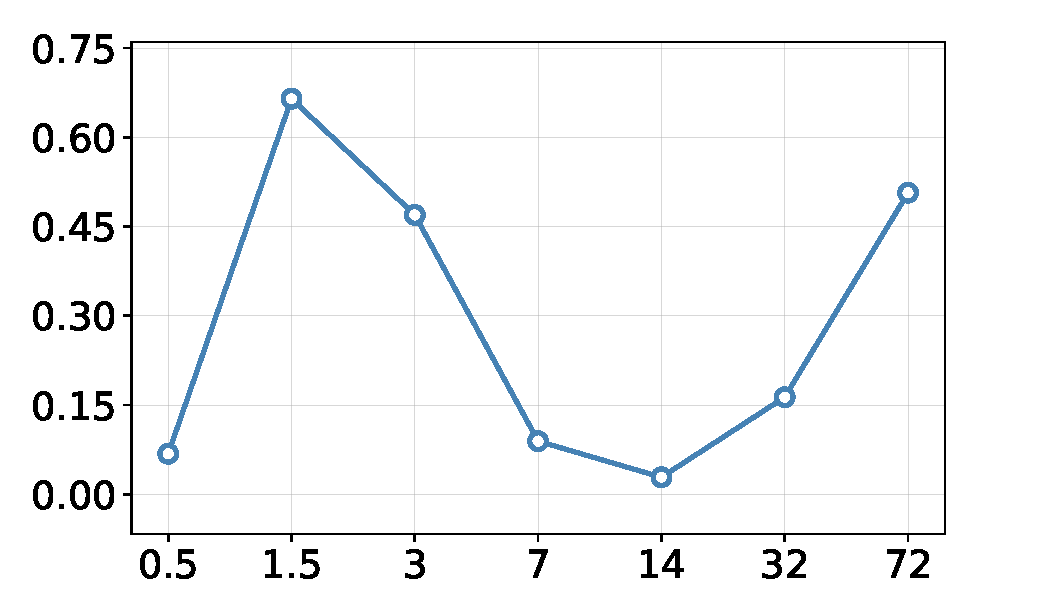
\includegraphics[width=\linewidth]{Figures_Qwen_scaling/Multi-subject-RLVR__mean.pdf}
%             \caption{Multi-subject}
%             \label{fig:sub1}
%         \end{subfigure}
%         \hfill
%         \begin{subfigure}{0.19\textwidth}
%             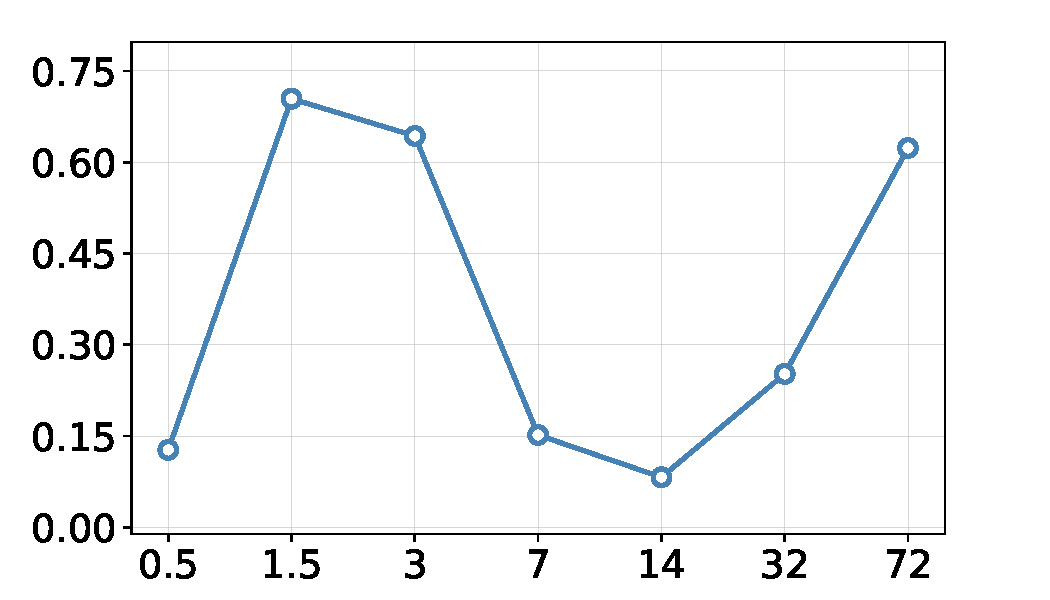
\includegraphics[width=\linewidth]{Figures_Qwen_scaling/Natural_Reasoning__mean.pdf}
%             \caption{NaturalReasoning}
%             \label{fig:sub2}
%         \end{subfigure}
%     % \end{minipage}
%     \begin{subfigure}{0.19\textwidth}
%         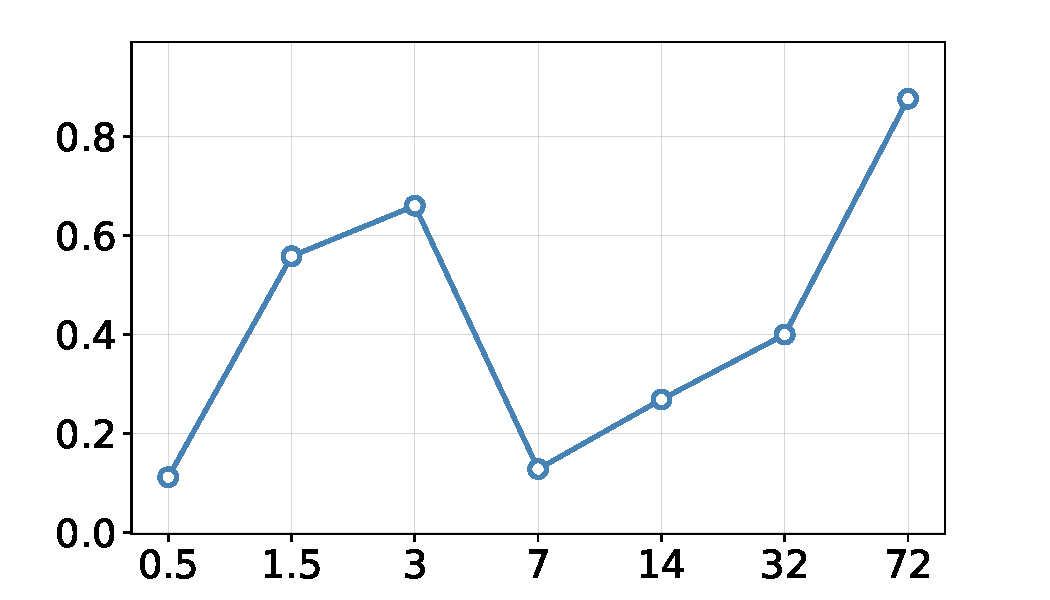
\includegraphics[width=\linewidth]{Figures_Qwen_scaling/GSM8k__mean.pdf}
%         \caption{GSM8K}
%         \label{fig:sub3}
%     \end{subfigure}
%     \hfill
%     \begin{subfigure}{0.19\textwidth}
%         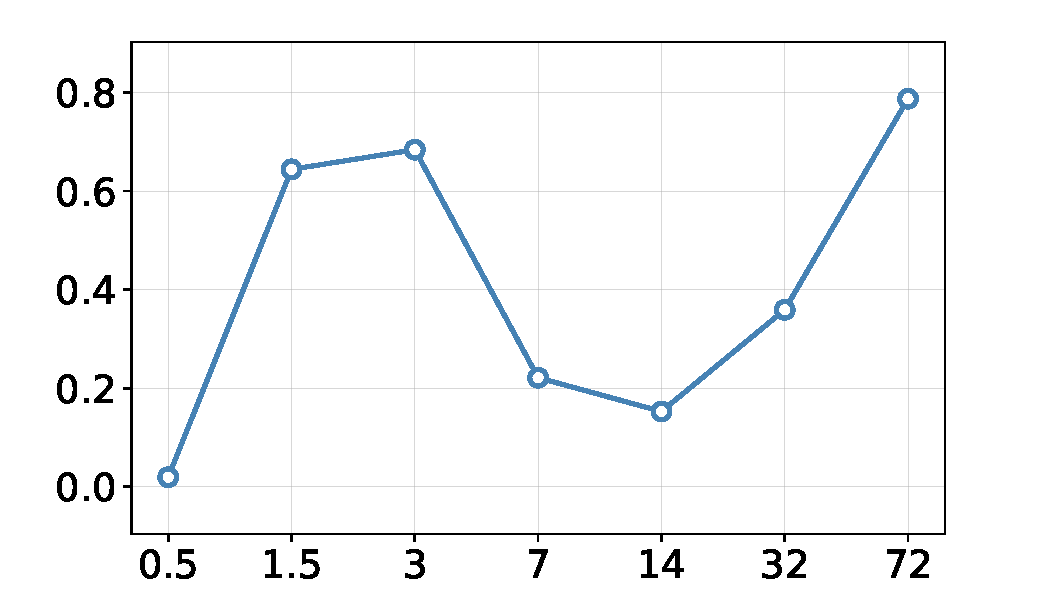
\includegraphics[width=\linewidth]{Figures_Qwen_scaling/MATH__mean.pdf}
%         \caption{MATH}
%         \label{fig:sub4}
%     \end{subfigure}
%     \hfill
%     \begin{subfigure}{0.19\textwidth}
%         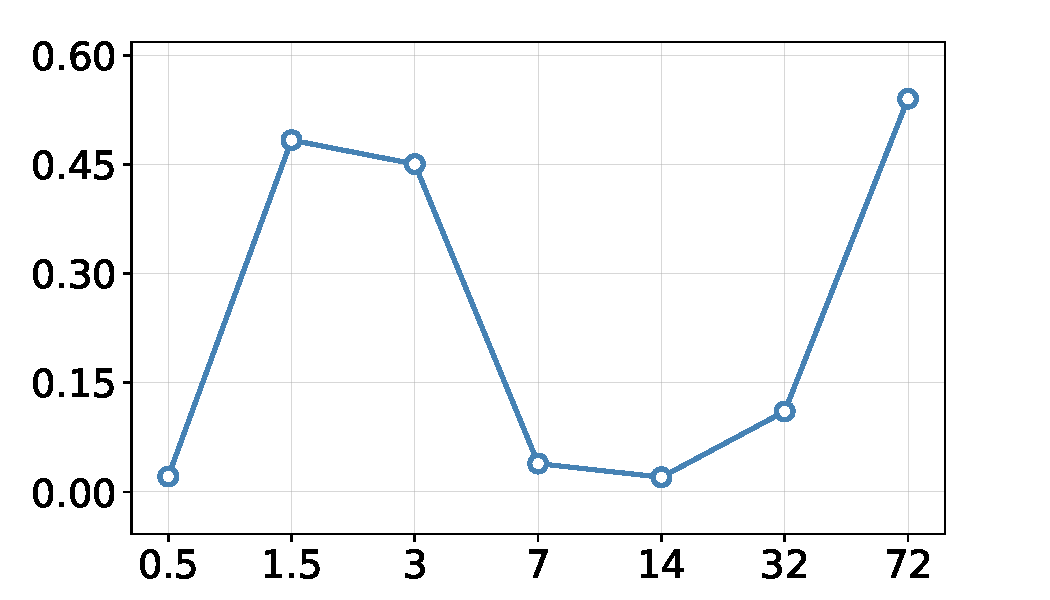
\includegraphics[width=\linewidth]{Figures_Qwen_scaling/AIME1983-2024__mean.pdf}
%         \caption{AIME}
%         \label{fig:sub5}
%     \end{subfigure}
%     \vspace{-1.2mm}
    
%     \caption{\textbf{Scaling Behaviour of False positive rate (FPR).}  We evaluate the FPRs of the Qwen2.5-Instruct model series (with sizes 0.5B, 1.5B, 3B, 7B, 14B, 32B, and 72B) and analyze how FPR varies with model size. In each figure, the caption specifies the evaluation dataset (as in Table~\ref{tab:merged-five}); the x-axis is the model size (B) and the y-axis is the FPR averaged over the ten ``master keys'' in Table~\ref{tab:merged-five}.}
%     \label{fig:Qwen-scaling-main}
% \end{figure}

\paragraph{The Scaling Behaviour of False Positive Rate. }

    \begin{figure}[htbp]
    \vspace{-2mm}

    \centering
    % First row (2 centered subfigures)
    \begin{minipage}{0.70\textwidth} 
        \centering
        \begin{subfigure}{0.33\textwidth}
            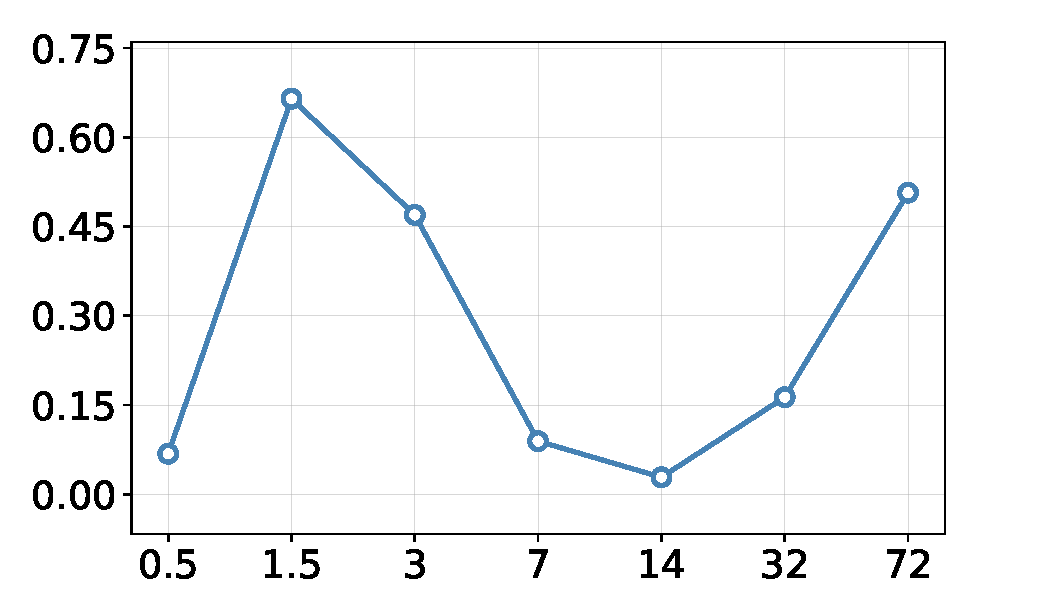
\includegraphics[width=\linewidth]{Figures_Qwen_scaling/Multi-subject-RLVR__mean.pdf}
            \caption{Multi-subject RLVR}
            \label{fig:sub1}
        \end{subfigure}
        % \hfill
        \hspace{2em}
        \begin{subfigure}{0.33\textwidth}
            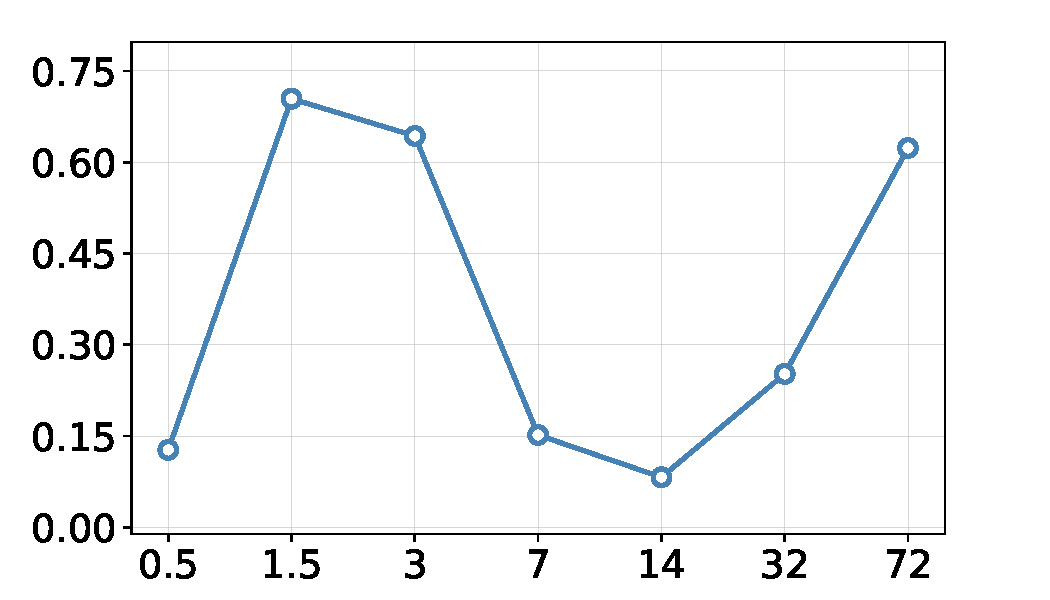
\includegraphics[width=\linewidth]{Figures_Qwen_scaling/Natural_Reasoning__mean.pdf}
            \caption{NaturalReasoning}
            \label{fig:sub2}
        \end{subfigure}
    \end{minipage}


    \vspace{0.5em} % 
    
    % second row (3)
    \begin{subfigure}{0.225\linewidth}
        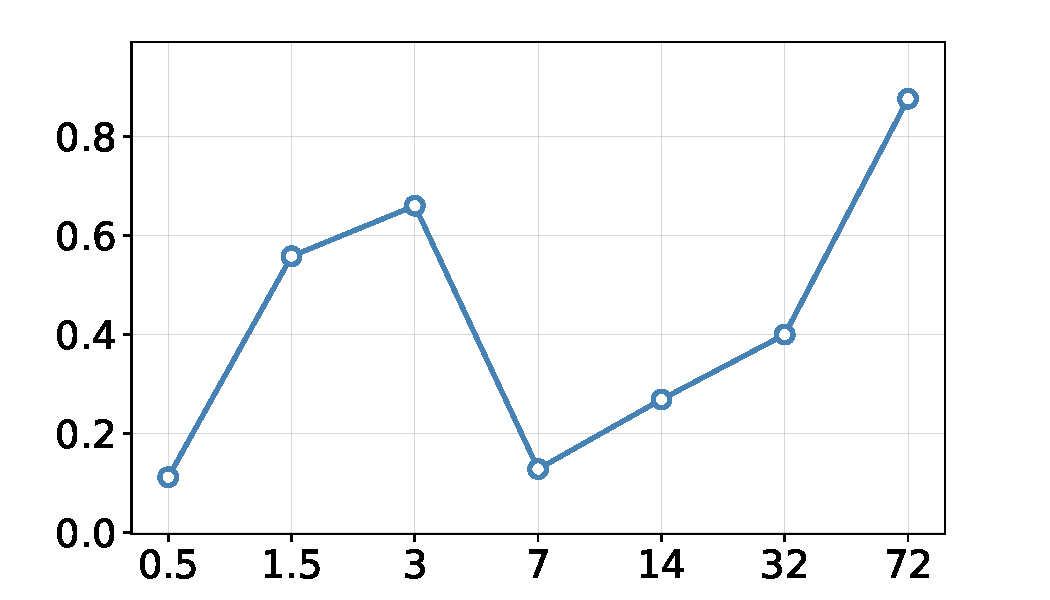
\includegraphics[width=\linewidth]{Figures_Qwen_scaling/GSM8k__mean.pdf}
        \caption{GSM8K}
        \label{fig:sub3}
    \end{subfigure}
    % \hfill
    \begin{subfigure}{0.225\linewidth}
        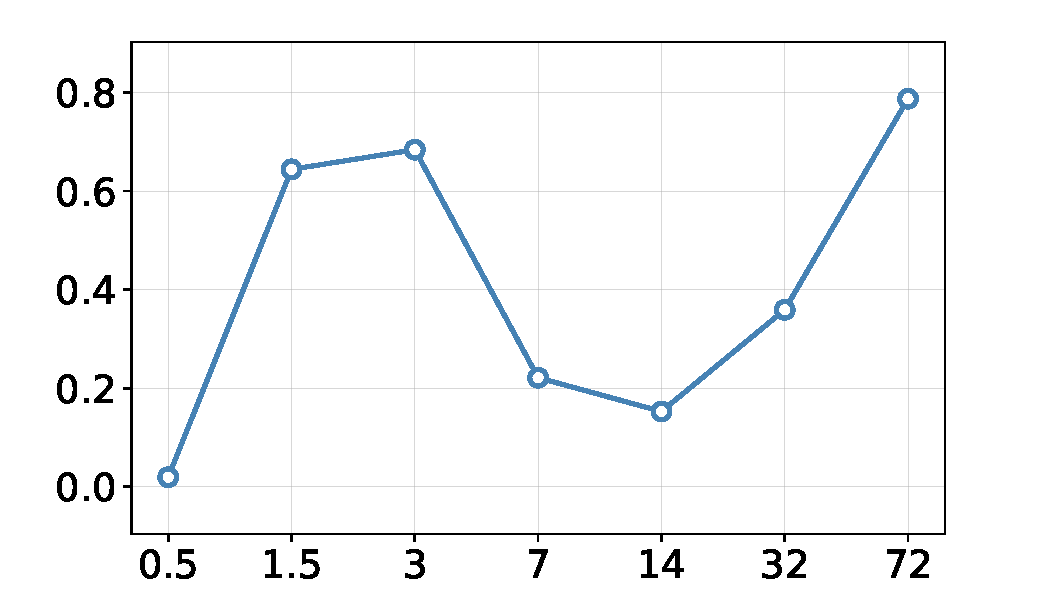
\includegraphics[width=\linewidth]{Figures_Qwen_scaling/MATH__mean.pdf}
        \caption{MATH}
        \label{fig:sub4}
    \end{subfigure}
    % \hfill
    \begin{subfigure}{0.225\linewidth}
        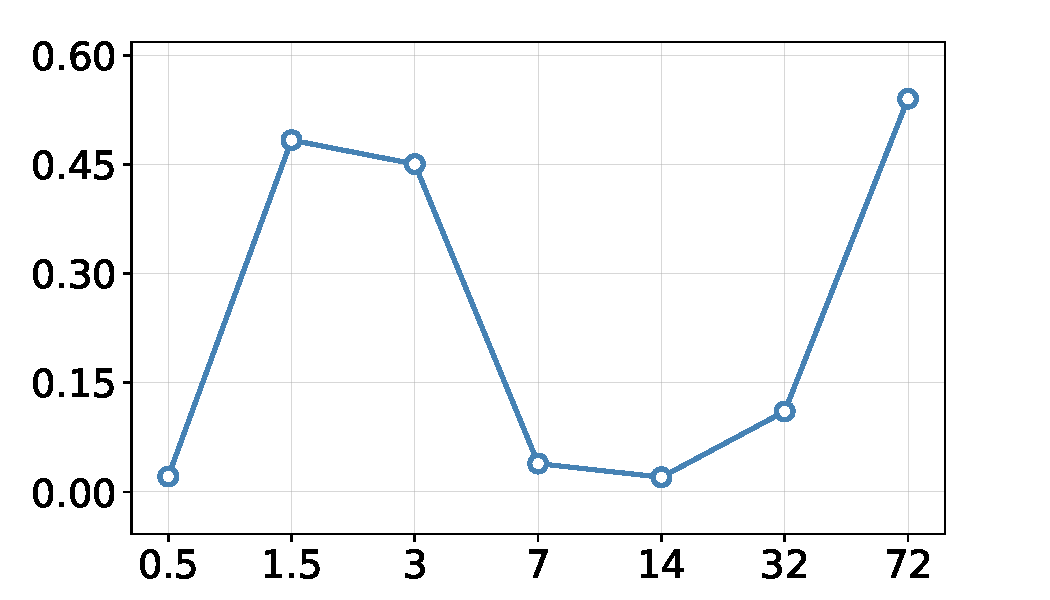
\includegraphics[width=\linewidth]{Figures_Qwen_scaling/AIME1983-2024__mean.pdf}
        \caption{AIME}
        \label{fig:sub5}
    \end{subfigure}
    \vspace{-2mm}
    \caption{\textbf{False Positive Rate (FPR) versus scaling of Qwen models.}  We analyze how FPR varies with model size using Qwen2.5-Instruct model series. 
    % (with sizes 0.5B, 1.5B, 3B, 7B, 14B, 32B, and 72B). 
    All subfigures use X-axis as model size (B) and use y-axis as FPR averaged over all ``master keys''.}
    \label{fig:Qwen-scaling-main}
    \vspace{-1em}
\end{figure}


We examine the scaling behavior of the Qwen2.5-Instruct model family (ranging from 0.5B to 72B parameters) across multiple benchmarks. Figure~\ref{fig:Qwen-scaling-main} reports the averaged scaling trend over the ten ''master keys” listed in Table~\ref{tab:merged-five}.  Surprisingly, the scaling patterns are consistent across all datasets and ``master keys'', but exhibit a non-monotonic trend. The 0.5B model achieves the lowest FPR but also shows the weakest alignment with GPT-4o (Table~\ref{tab:consistency}). As the model size increases to 1.5–3B, FPR rises sharply while consistency improves. Performance reaches its peak at 7–14B, balancing low FPR with high consistency, before FPR climbs again at the largest scales of 32B and 72B. While fully elucidating the underlying mechanism remains outside our current scope, we discuss a preliminary hypothesis in Appendix~\ref{app:hall_scal}.


% In this section, we plot the scaling behavior of the Qwen2.5-Instruct model series (0.5B, 1.5B, 3B, 7B, 14B, 32B, 72B) across various ``master key'' responses and benchmarks. Figure~\ref{fig:ten_multi_sub} illustrates the scaling trends on the Multi-subject RLVR benchmark, while Figures~\ref{fig:ten_natural_reason}, \ref{fig:ten_gsm8k}, \ref{fig:ten_math}, and \ref{fig:ten_aime} show results for the NaturalReasoning, GSM8K, MATH, and AIME1983–2024 benchmarks, respectively.

% Across all benchmarks and responses, we observe a consistent non-monotonic scaling pattern: false positive rates initially rise from 0.5B to 1.5B and 3B, decrease at 7B and 14B, and rise again at 32B and 72B.

% We analyze how FPR varies with model size across the Qwen2.5-Instruct series, as shown in Figure \ref{fig:Qwen-scaling}. Surprisingly, the scaling behavior is consistent for all datasets but non-monotonic. The 0.5 B model exhibits the lowest FPR rate but also the weakest agreement with GPT-4o (Table~\ref{tab:consistency}). As model size increases to 1.5–3 B, FPR rises sharply while consistency improves. Performance then peaks at 7–14 B, achieving both low FPR and high consistency, before FPR increases again at the largest scales of 32 B and 72 B. 

% We hypothesize the following mechanisms: (1) $0.5$ B (literal matcher): With limited knowledge, the model relies on surface-level string differences and therefore outputs NO whenever obvious mismatches appear, yielding lower FPR but many disagreements with GPT-4o.
% (2) $1.5$ B/$3$ B (coarse semantic matcher): These models possess just enough capacity to detect embedding-level similarity (e.g., shared units, symbols, or synonyms), yet lack fine-grained verification; as a result, they tend to over-predict \texttt{YES} and produce frequent false positive judgments.
% (3) $7$ B/$14$ B (calibrated verifier): Sufficient capacity enables precise comparison while retained caution suppresses unwarranted YES responses, producing the best overall trade-off.
% (4) $32$ B/$72$ B (self-solver):  An observation was made that Claude-4 sometimes deviates from the provided instruction to compare a given solution with a reference answer. Instead, it solves the question independently and subsequently compares the reference answer to its own derived solution. While this behavior is infrequently observed in other models, we hypothesize that the increased false positive rate in larger models is attributable to their inherent tendency to solve the question themselves before comparing the reference answer to their own derivation, rather than the provided solution. As a partial validation of this hypothesis, we discovered that removing the question from the prompt (i.e., providing only a response and a reference answer for evaluation) significantly reduces the FPR. This effect is particularly pronounced in large models (see Appendix \ref{app:remove} for further details). We leave the further investigation of the mechanism behind this scaling behavior as a direction for future work.


% \vspace{-5mm}

\paragraph{Automatic Discovery of New Master Keys. }
\label{sec:key_gene}
We also find that text embedding–similar to our “master keys” can trigger high false positive rates. For example, “mental process,” which is embedding-similar to the master key “Thought process:”, induces a 16.1\% false positive rate for GPT-4o on GSM8K dataset. More details are provided in Appendix~\ref{app:key_gene}.

\begin{table}[htbp]
    \centering
    % 第一个表格的 minipage
   \begin{subtable}{0.46\textwidth}
        \centering
        \small
        \resizebox{\linewidth}{!}{%
        \begin{tabular}{l*{2}{r@{\,$\mid$\,}l r@{\,$\mid$\,}l}}
        \toprule
        & \multicolumn{4}{c}{Qwen2.5-72B}
        & \multicolumn{4}{c}{Qwen2.5-7B} \\
        \cmidrule(lr){2-5}
        \cmidrule(lr){6-9}
        Dataset
        & \multicolumn{2}{c}{CoT}   & \multicolumn{2}{c}{No-CoT}
        & \multicolumn{2}{c}{CoT}   & \multicolumn{2}{c}{No-CoT} \\
        \midrule
        Multi-subject RLVR
          & \textbf{5.3} & \textbf{10.7} & 51.4 & 70.5
          & 34.6 & 53.0   & \textbf{9.0} & \textbf{15.7} \\
        NaturalReasoning
          & \textbf{34.5} & \textbf{55.4} & 62.3 & 72.8
          & 23.9 & 31.6    & \textbf{15.2} & \textbf{23.2} \\
        GSM8K
          & 95.5 & 97.0    & \textbf{87.6} & \textbf{90.9}
          & 87.6 & 91.3    & \textbf{12.8} & \textbf{25.4} \\
        MATH
          & 81.0 & \textbf{85.2} & \textbf{78.7} & 88.6
          & 51.6 & 59.9           & \textbf{22.1} & \textbf{31.0} \\
        AIME 1983--2024
          & \textbf{38.1} & \textbf{47.3} & 54.0 & 90.9
          & 4.2  & \textbf{6.9}          & \textbf{3.9} & 8.6 \\
        \midrule
        Overall
          & \textbf{50.9} & 97.0 & 66.8 & \textbf{90.9}
          & 40.4 & 91.3        & \textbf{12.6} & \textbf{31.0} \\
        \bottomrule
        \end{tabular}
        }
        \caption{}
        \label{tab:fpr_cot_aligned_qwen}
    \end{subtable}
    \hfill % 在两个 minipage 之间填充空白
    % 第二个表格的 minipage
    \begin{subtable}{0.50\textwidth}
        \centering
        \small
        \renewcommand{\arraystretch}{1.30}
        \resizebox{\linewidth}{!}{%
                \begin{tabular}{lcccc}
        \toprule
        & \multicolumn{2}{c}{Qwen2.5-72B} & \multicolumn{2}{c}{Qwen2.5-7B} \\
        \cmidrule(lr){2-3} \cmidrule(lr){4-5}
        Dataset & Standard & NQ & Standard & NQ \\
        \midrule
        Multi-subject RLVR & $51.4\mid70.5$ & $\mathbf{4.9}\mid\mathbf{10.8}$  & $9.0\mid15.7$  & $\mathbf{0.2}\mid\mathbf{0.8}$ \\
        NaturalReasoning   & $62.3\mid72.8$ & $\mathbf{50.1}\mid\mathbf{62.4}$ & $15.2\mid23.2$ & $\mathbf{2.3}\mid\mathbf{4.2}$ \\
        GSM8K              & $87.6\mid90.9$ & $\mathbf{0.0}\mid\mathbf{0.0}$   & $12.8\mid25.4$ & $\mathbf{0.7}\mid\mathbf{4.8}$ \\
        MATH               & $78.7\mid88.6$ & $\mathbf{2.8}\mid\mathbf{6.8}$   & $22.1\mid31.0$ & $\mathbf{6.1}\mid\mathbf{22.2}$ \\
        AIME 1983--2024    & $54.0\mid90.9$ & $\mathbf{0.0}\mid\mathbf{0.0}$   & $3.9\mid8.6$   & $\mathbf{0.0}\mid\mathbf{0.0}$ \\
        \bottomrule
        \end{tabular}
        }
        \caption{}
        \label{tab:fpr_nq_main}
    \end{subtable}
    \vspace{-2mm} % 根据需要调整表格与标题的间距
    \caption{\textbf{Effects of inference-time techniques and removing questions from prompts on FPRs (\%).} 
    \textbf{(Left)} \textbf{Inference-time techniques may increase FPRs:} We compare Average$\mid$Worst FPRs using CoT prompting and majority voting (CoT) versus non-CoT prompting (No-CoT). 
    % For each dataset/model pair, the lower value is bold. 
    \textbf{(Right)} \textbf{No-question evaluation prompts lead to lower FPRs:} We compare the Average$\mid$Worst FPRs using the standard prompt versus its no-question version (NQ). }
    \vspace{-2pt}
\end{table}

\paragraph{Inference-time Strategies Fail to Enhance the Robustness.}
% Generative reward models can be enhanced with inference-time techniques such as chain-of-thought (CoT) prompting and majority voting. While \citet{zhang2024generative} studies these methods in a reference-free setting, we evaluate them in a reference-based setting where the model also sees the ground-truth answer. We adapt our prompt to a CoT style (cf. Table~\ref{tab:fpr_cot_aligned_qwen}), sample five responses per input, and use majority voting for the final judgment, comparing the false positive rate of  CoT+voting against standard greedy decoding without CoT prompting (Table~\ref{tab:fpr_cot_aligned}). We find that inference-time techniques usually reduce false positives on general reasoning benchmarks, but their effect on mathematical benchmarks is mixed, hurting Qwen models while often helping LLaMA models. Overall, their benefits in the reference-based setting are highly model- and domain-dependent and should therefore be used with caution. More details can be found in Appendix~\ref{app:cot}.
\citet{zhang2024generative} show that inference-time techniques such as chain-of-thought (CoT) and majority voting can enhance generative reward models in a reference-free setting. However, in Table~\ref{tab:fpr_cot_aligned_qwen}, we found that using the CoT prompt and majority voting for five generations (the CoT column) can have worse performance compared with the non-COT prompt (the No-CoT column) in our reference-based setting. More discussion is provided in Appendix~\ref{app:cot}, where we show that inference-time techniques are not reliable in all cases and should be applied with caution.







% \begin{table}[htbp]
% \centering
% \small
% \resizebox{0.5\textwidth}{!}{%
% \begin{tabular}{l*{2}{r@{\,$\mid$\,}l r@{\,$\mid$\,}l}}
% \toprule
% & \multicolumn{4}{c}{Qwen2.5-72B}
% & \multicolumn{4}{c}{Qwen2.5-7B} \\
% \cmidrule(lr){2-5}
% \cmidrule(lr){6-9}
% Dataset
% & \multicolumn{2}{c}{CoT}   & \multicolumn{2}{c}{No-CoT}
% & \multicolumn{2}{c}{CoT}   & \multicolumn{2}{c}{No-CoT} \\
% \midrule
% Multi-subject RLVR
%   & \textbf{5.3} & \textbf{10.7} & 51.4 & 70.5
%   & 34.6 & 53.0   & \textbf{9.0} & \textbf{15.7} \\
% NaturalReasoning
%   & \textbf{34.5} & \textbf{55.4} & 62.3 & 72.8
%   & 23.9 & 31.6    & \textbf{15.2} & \textbf{23.2} \\
% GSM8K
%   & 95.5 & 97.0    & \textbf{87.6} & \textbf{90.9}
%   & 87.6 & 91.3    & \textbf{12.8} & \textbf{25.4} \\
% MATH
%   & 81.0 & \textbf{85.2} & \textbf{78.7} & 88.6
%   & 51.6 & 59.9           & \textbf{22.1} & \textbf{31.0} \\
% AIME 1983--2024
%   & \textbf{38.1} & \textbf{47.3} & 54.0 & 90.9
%   & 4.2  & \textbf{6.9}          & \textbf{3.9} & 8.6 \\
% \midrule
% Overall
%   & \textbf{50.9} & 97.0 & 66.8 & \textbf{90.9}
%   & 40.4 & 91.3        & \textbf{12.6} & \textbf{31.0} \\
% \bottomrule
% \end{tabular}
% }
% \caption{\textbf{Add inference-time techniques can increase FPRs.} We compare Average$\mid$Worst FPRs (\%) under CoT prompting with majority voting (CoT) versus a non-CoT prompt (No-CoT). For each dataset--model pair, the lower value between CoT and No-CoT is shown in bold.}
% \label{tab:fpr_cot_aligned_qwen}
% \vspace{-5mm}
% \end{table}

\paragraph{Removing Questions Reduces False Positives. }
We compare the standard reference-based prompt to a no-question variant (NQ) that includes only the response and reference answer in Table \ref{tab:fpr_nq_main}. Removing the question sharply reduces FPR. Consequently, we recommend omitting the question when evaluating math tasks, but we caution that general reasoning often requires the questions for judgment. Details are deferred to Appendix~\ref{app:remove}.


% \begin{table}[H]
% \centering
% \begin{adjustbox}{max width=\linewidth}
% \begin{tabular}{lcccc}
% \toprule
% & \multicolumn{2}{c}{Qwen2.5-72B} & \multicolumn{2}{c}{Qwen2.5-7B} \\
% \cmidrule(lr){2-3} \cmidrule(lr){4-5}
% Dataset & Standard & NQ & Standard & NQ \\
% \midrule
% Multi-subject RLVR & $51.4\mid70.5$ & $\mathbf{4.9}\mid\mathbf{10.8}$  & $9.0\mid15.7$  & $\mathbf{0.2}\mid\mathbf{0.8}$ \\
% NaturalReasoning   & $62.3\mid72.8$ & $\mathbf{50.1}\mid\mathbf{62.4}$ & $15.2\mid23.2$ & $\mathbf{2.3}\mid\mathbf{4.2}$ \\
% GSM8K              & $87.6\mid90.9$ & $\mathbf{0.0}\mid\mathbf{0.0}$   & $12.8\mid25.4$ & $\mathbf{0.7}\mid\mathbf{4.8}$ \\
% MATH               & $78.7\mid88.6$ & $\mathbf{2.8}\mid\mathbf{6.8}$   & $22.1\mid31.0$ & $\mathbf{6.1}\mid\mathbf{22.2}$ \\
% AIME 1983--2024    & $54.0\mid90.9$ & $\mathbf{0.0}\mid\mathbf{0.0}$   & $3.9\mid8.6$   & $\mathbf{0.0}\mid\mathbf{0.0}$ \\
% \bottomrule
% \end{tabular}
% \end{adjustbox}
% \caption{\textbf{Removing question from the evaluation prompt helps to reduce FPRs.} We compare the Average$\mid$Worst FPRs (\%) with the standard prompt (Standard) versus its no-question variant (NQ). The lower value between standard and NQ is bold.}
% \label{tab:fpr_nq_main}
% \end{table}


% \begin{table}[H]
% \centering
% \begin{adjustbox}{max width=1.5\textwidth}
% \begin{tabular}{lcccc}
% \toprule
% & \multicolumn{2}{c}{Qwen2.5-72B} & \multicolumn{2}{c}{Qwen2.5-7B} \\
% \cmidrule(lr){2-3} \cmidrule(lr){4-5}
% Dataset & Standard & NQ & Standard & NQ \\
% \midrule
% Multi-subject RLVR & $51.4\mid70.5$ & $\,\,\,4.9\mid10.8$  & $\,\,\,9.0\mid15.7$  & $0.2\mid0.8$ \\
% NaturalReasoning   & $62.3\mid72.8$ & $50.1\mid62.4$ & $15.2\mid23.2$ & $2.3\mid4.2$ \\
% GSM8K              & $87.6\mid90.9$ & $0.0\mid0.0$   & $12.8\mid25.4$ & $0.7\mid4.8$ \\
% MATH               & $78.7\mid88.6$ & $2.8\mid6.8$   & $22.1\mid31.0$ & $\,\,\,6.1\mid22.2$ \\
% AIME 1983--2024    & $54.0\mid90.9$ & $0.0\mid0.0$   & $3.9\mid8.6$   & $0.0\mid0.0$ \\
% \bottomrule
% \end{tabular}
% \caption{\textbf{Removing question from the evaluation prompt helps to reduce FPRs.} We compare the Average$\mid$Worst FPRs (\%) with the standard prompt (Standard) versus its no-question variant (NQ).}
% \label{tab:fpr_nq_main}
% \end{adjustbox}
% \end{table}


% To validate this, we construct a corpus and usie all-MiniLM-L6-v2~\citep{reimers-2019-sentence-bert} to retrieve the two nearest neighbors of each key by cosine similarity. 



% In this subsection, we study whether adversarial ``master keys'' can be systematically expanded. To this end, we build a corpus of $\sim$1.5M short sentences from public datasets, encode all sentences together with the three English ``master keys'' using all-MiniLM-L6-v2~\citep{reimers-2019-sentence-bert}, and retrieve the two nearest neighbors of each key by cosine similarity. We then evaluate the false positive rates (FPRs) of these neighbors for GPT-4o.  
% % Further details on corpus construction and the complete list of identified neighbors can be found in Appendix~\ref{app:key_gene}.

% Table~\ref{tab:new-key-main} reports the average FPRs elicited in GPT-4o by the nearest neighbors of each of the three original ``master keys'' (cf. Table~\ref{tab:merged-five}). The results demonstrate that sentences with high embedding similarity to the original keys remain highly adversarial, indicating that the vulnerability is not limited to \textbf{a few} specific phrases but extends to a broader neighborhood in the embedding space.




% \subsection{Inference-time Strategies Fail to enhance the robustness}
% Generative reward models can be enhanced with inference-time techniques such as chain-of-thought (CoT) prompting and majority voting. While \citet{zhang2024generative} studies these methods in a reference-free setting, we evaluate them in a reference-based setting where the model also sees the ground-truth answer. We adapt our prompt to a CoT style (cf. Table~\ref{tab:appendix:grade_template_cot}), sample five responses per input, and use majority voting for the final judgment, comparing the false positive rate of  CoT+voting against standard greedy decoding without CoT prompting (Table~\ref{tab:fpr_cot_aligned}). We find that inference-time techniques usually reduce false positives on general reasoning benchmarks, but their effect on mathematical benchmarks is mixed, hurting Qwen models while often helping LLaMA models. Overall, their benefits in the reference-based setting are highly model- and domain-dependent and should therefore be used with caution. More details can be found in Appendix~\ref{app:cot}.

% \begin{table*}[t]
% \centering
% \small
% \resizebox{.9\textwidth}{!}{%
% \begin{tabular}{l*{4}{r@{\,$\mid$\,}l r@{\,$\mid$\,}l}}
% \toprule
% & \multicolumn{4}{c}{Qwen2.5-72B}
% & \multicolumn{4}{c}{Qwen2.5-7B}
% & \multicolumn{4}{c}{LLaMA3-70B}
% & \multicolumn{4}{c}{LLaMA3-8B} \\
% \cmidrule(lr){2-5}
% \cmidrule(lr){6-9}
% \cmidrule(lr){10-13}
% \cmidrule(lr){14-17}
% % Dataset (Avg$\mid$Worst FPR)
% Dataset
% & \multicolumn{2}{c}{CoT}   & \multicolumn{2}{c}{No-CoT}
% & \multicolumn{2}{c}{CoT}   & \multicolumn{2}{c}{No-CoT}
% & \multicolumn{2}{c}{CoT}   & \multicolumn{2}{c}{No-CoT}
% & \multicolumn{2}{c}{CoT}   & \multicolumn{2}{c}{No-CoT} \\
% \midrule
% Multi-subject RLVR
%   & \textbf{5.3} & \textbf{10.7} & 51.4 & 70.5
%   & 34.6 & 53.0   & \textbf{9.0} & \textbf{15.7}
%   & \textbf{43.4} & \textbf{59.6} & 66.2 & 79.7
%   & \textbf{30.8} & \textbf{45.3} & 55.0 & 73.8 \\
% NaturalReasoning
%   & \textbf{34.5} & \textbf{55.4} & 62.3 & 72.8
%   & 23.9 & 31.6    & \textbf{15.2} & \textbf{23.2}
%   & \textbf{66.8} & \textbf{80.1}  & 76.6 & 82.9
%   & \textbf{48.4} & \textbf{61.5}  & 83.0 & 86.7 \\
% GSM8K
%   & 95.5 & 97.0    & \textbf{87.6} & \textbf{90.9}
%   & 87.6 & 91.3    & \textbf{12.8} & \textbf{25.4}
%   & 96.7 & 97.0    & \textbf{83.4} & \textbf{89.2}
%   & \textbf{77.9} & \textbf{79.5}  & 79.1 & 88.3 \\
% MATH
%   & 81.0 & \textbf{85.2} & \textbf{78.7} & 88.6
%   & 51.6 & 59.9           & \textbf{22.1} & \textbf{31.0}
%   & \textbf{82.8} & \textbf{84.9} & 87.7 & 92.4
%   & \textbf{42.5} & \textbf{48.9} & 85.6 & 91.2 \\
% AIME 1983--2024
%   & \textbf{38.1} & \textbf{47.3} & 54.0 & 90.9
%   & 4.2  & \textbf{6.9}          & \textbf{3.9} & 8.6
%   & \textbf{57.4} & \textbf{66.5} & 89.1 & 95.1
%   & \textbf{7.9}  & \textbf{11.0} & 82.0 & 92.0 \\
% \midrule
% Overall
%   & \textbf{50.9} & 97.0 & 66.8 & \textbf{90.9}
%   & 40.4 & 91.3        & \textbf{12.6} & \textbf{31.0}
%   & \textbf{69.4} & 97.0 & 80.6 & \textbf{95.1}
%   & \textbf{41.5} & \textbf{79.5} & 76.9 & 92.0 \\
% \bottomrule
% \end{tabular}
% }%
% \caption{\textbf{Average$\mid$Worst FPRs (\%) with and without inference-time techniques.} For each dataset-model pair, the lower value between CoT and No-CoT is shown in bold.}
% \label{tab:fpr_cot_aligned}
% \end{table*}



% \subsection{Removing Questions from Prompts Reduces False Positives}
% \label{sec:remove}

% We investigate the impact of prompt templates on FPRs by comparing the standard reference-based prompt (Standard) with a variant that only includes the "response" and the "reference answer", omitting the "question" (NQ).
% Table~\ref{tab:fpr_nq_main} reports the average and worst-case FPRs across all identified ``master keys''. The results demonstrate that removing the question substantially reduces FPRs, particularly on math benchmarks (GSM8K, MATH, AIME), where false positives are often eliminated entirely. Consequently, we recommend omitting the question when evaluating math tasks. However, this strategy should be applied with caution in general reasoning, where the problem statement is often essential for determining answer equivalence in open-ended contexts. More details can be found in Appendix~\ref{app:remove}.

% \begin{table*}[t]
% \centering
% \small
% \begin{tabular}{lcccc}
% \toprule
% & \multicolumn{2}{c}{Qwen2.5-72B} & \multicolumn{2}{c}{Qwen2.5-7B} \\
% \cmidrule(lr){2-3} \cmidrule(lr){4-5}
% Dataset & Standard & NQ & Standard & NQ \\
% \midrule
% Multi-subject RLVR & $51.4\mid70.5$ & $\,\,\,4.9\mid10.8$  & $\,\,\,9.0\mid15.7$  & $0.2\mid0.8$ \\
% NaturalReasoning   & $62.3\mid72.8$ & $50.1\mid62.4$ & $15.2\mid23.2$ & $2.3\mid4.2$ \\
% GSM8K              & $87.6\mid90.9$ & $0.0\mid0.0$   & $12.8\mid25.4$ & $0.7\mid4.8$ \\
% MATH               & $78.7\mid88.6$ & $2.8\mid6.8$   & $22.1\mid31.0$ & $\,\,\,6.1\mid22.2$ \\
% AIME 1983--2024    & $54.0\mid90.9$ & $0.0\mid0.0$   & $3.9\mid8.6$   & $0.0\mid0.0$ \\
% \bottomrule
% \end{tabular}
% \caption{\textbf{Removing question from the evaluation prompt helps to reduce FPRs.} We compare the Average$\mid$Worst FPRs (\%) with the standard prompt (Standard) versus its no-question variant (NQ).}
% \label{tab:fpr_nq_main}
% \end{table*}



% \textbf{Additional Experimental Results.} We present further analytical experiments in the appendix. Appendix~\ref{app:cot} examines inference-time techniques like chain-of-thought and majority voting, finding that they do not reduce the false positive rate of generative reward models, and may even increase it. Finally, Appendix~\ref{app:remove} shows that removing the original question from the prompt can substantially reduce false positive rates, particularly for larger models.